\documentclass[11pt,a4paper]{article}

% ========== PAQUETES ==========
\usepackage[utf8]{inputenc}
\usepackage[spanish]{babel}
\usepackage[T1]{fontenc}
\usepackage{lmodern}
\usepackage{microtype}

% Geometría y márgenes
\usepackage[margin=2.5cm, top=3cm, bottom=3cm]{geometry}

% Colores y gráficos
\usepackage{xcolor}
\usepackage{graphicx}
\usepackage{tikz}
\usepackage{circuitikz}
\usepackage{tcolorbox}
\usepackage{float}
\usepackage{booktabs}
\usepackage{array}

% Para código
\usepackage{listings}
\usepackage{color}

% Fuentes y tipografía
\usepackage{titlesec}
\usepackage{fancyhdr}
\graphicspath{{./figures/}}

% Enlaces y referencias
\usepackage[colorlinks=true, linkcolor=darkblue, urlcolor=darkblue, citecolor=darkblue]{hyperref}

% Matemáticas y código
\usepackage{amsmath, amssymb, amsthm}

% Listas y enumeraciones
\usepackage{enumitem}

% ========== DEFINICIÓN DE COLORES ==========
\definecolor{primarycolor}{RGB}{41, 128, 185}    % Azul elegante
\definecolor{secondarycolor}{RGB}{52, 73, 94}    % Gris azulado
\definecolor{accentcolor}{RGB}{231, 76, 60}      % Rojo acento
\definecolor{lightgray}{RGB}{236, 240, 241}      % Gris claro
\definecolor{darkblue}{RGB}{25, 42, 86}          % Azul oscuro
\definecolor{successcolor}{RGB}{46, 204, 113}    % Verde éxito

% ========== CONFIGURACIÓN DE TÍTULOS ==========
\titleformat{\section}
  {\Large\bfseries\color{primarycolor}}
  {\thesection}{1em}{}

\titleformat{\subsection}
  {\large\bfseries\color{secondarycolor}}
  {\thesubsection}{1em}{}

\titleformat{\subsubsection}
  {\normalsize\bfseries\color{secondarycolor}}
  {\thesubsubsection}{1em}{}

% ========== CONFIGURACIÓN DE HEADER Y FOOTER ==========
\pagestyle{fancy}
\fancyhf{}
\fancyhead[L]{\textcolor{secondarycolor}{\small\leftmark}}
\fancyhead[R]{\textcolor{secondarycolor}{\small Página \thepage}}
\fancyfoot[C]{\textcolor{primarycolor}{\rule{0.3\textwidth}{0.4pt}}}
\renewcommand{\headrulewidth}{0.5pt}
\renewcommand{\headrule}{\hbox to\headwidth{\color{primarycolor}\leaders\hrule height \headrulewidth\hfill}}

% ========== CAJAS DE TEXTO PERSONALIZADAS ==========
\tcbuselibrary{skins,breakable}

% Caja de información
\newtcolorbox{infobox}{
  enhanced,
  breakable,
  colback=lightgray,
  colframe=primarycolor,
  leftrule=4mm,
  rightrule=0mm,
  toprule=0mm,
  bottomrule=0mm,
  arc=0mm,
  outer arc=0mm,
  left=5mm,
  right=5mm,
  top=5mm,
  bottom=5mm
}

% Caja de advertencia
\newtcolorbox{warningbox}{
  enhanced,
  breakable,
  colback=orange!10,
  colframe=orange!80!red,
  leftrule=4mm,
  rightrule=0mm,
  toprule=0mm,
  bottomrule=0mm,
  arc=0mm,
  outer arc=0mm,
  left=5mm,
  right=5mm,
  top=5mm,
  bottom=5mm
}

% Caja de éxito
\newtcolorbox{successbox}{
  enhanced,
  breakable,
  colback=green!10,
  colframe=successcolor,
  leftrule=4mm,
  rightrule=0mm,
  toprule=0mm,
  bottomrule=0mm,
  arc=0mm,
  outer arc=0mm,
  left=5mm,
  right=5mm,
  top=5mm,
  bottom=5mm
}

% Caja de problema con título
\newtcolorbox{problembox}[1]{
  enhanced,
  breakable,
  colback=white,
  colframe=primarycolor,
  boxrule=1.5pt,
  arc=3mm,
  left=5mm,
  right=5mm,
  top=5mm,
  bottom=5mm,
  title={\centering\textcolor{white}{\textbf{#1}}},
  coltitle=white,
  colbacktitle=primarycolor,
  attach boxed title to top center={yshift=-2mm}
}

% ========== CONFIGURACIÓN DE LISTAS ==========
\setlist[itemize,1]{label=\textcolor{primarycolor}{$\bullet$}}
\setlist[itemize,2]{label=\textcolor{secondarycolor}{$\circ$}}
\setlist[enumerate]{label=\textcolor{primarycolor}{\arabic*.}}

% ========== CONFIGURACIÓN DE CÓDIGO MATLAB ==========
\lstdefinelanguage{Matlab}{
  basicstyle=\ttfamily\small,
  breaklines=true,
  deletekeywords={__},
  emph={[1]for, if, else, elseif, end, function, return},
  emphstyle={[1]\color{blue}\bfseries},
  emph={[2]mean, sqrt, sin, plot, figure, hold},
  emphstyle={[2]\color{blue}},
  identifierstyle=\color{black},
  keywordstyle=\color{blue}\bfseries,
  commentstyle=\color{gray}\ttfamily,
  stringstyle=\color{red},
  showstringspaces=false,
  morecomment=[l]\%,
  numbers=left,
  numberstyle=\tiny\color{gray},
  stepnumber=1,
  numbersep=5pt,
  frame=single,
  framexleftmargin=15pt,
  backgroundcolor=\color{lightgray},
  linewidth=\textwidth,
  literate={á}{{\'a}}1 {é}{{\'e}}1 {í}{{\'i}}1 {ó}{{\'o}}1 {ú}{{\'u}}1 
           {Á}{{\'A}}1 {É}{{\'E}}1 {Í}{{\'I}}1 {Ó}{{\'O}}1 {Ú}{{\'U}}1
           {à}{{\`a}}1 {è}{{\`e}}1 {ì}{{\`i}}1 {ò}{{\`o}}1 {ù}{{\`u}}1
           {ä}{{\"a}}1 {ë}{{\"e}}1 {ï}{{\"i}}1 {ö}{{\"o}}1 {ü}{{\"u}}1
           {â}{{\^a}}1 {ê}{{\^e}}1 {î}{{\^i}}1 {ô}{{\^o}}1 {û}{{\^u}}1
           {ã}{{\~a}}1 {õ}{{\~o}}1 {ñ}{{\~n}}1 {Ñ}{{\~N}}1
           {ç}{{\c{c}}}1 {Ç}{{\c{C}}}1
}

\lstset{language=Matlab}

% ========== INICIO DEL DOCUMENTO ==========
\begin{document}

% ========== PÁGINA DE TÍTULO PERSONALIZADA ==========
\begin{titlepage}
\thispagestyle{empty}

% Fondo colorido superior
\begin{tikzpicture}[remember picture, overlay]
  \fill[primarycolor] (current page.north west) rectangle ([yshift=-4cm]current page.north east);
\end{tikzpicture}

% Contenido del título
\vspace*{1cm}
\begin{center}
  {\Huge\bfseries\color{primarycolor} Problemas de Calidad Eléctrica}\\[0.8cm]
  {\Large\color{primarycolor}Grupo 5 - Itinerario de Eléctrica}\\[2cm]

  \vfill
  
  {\Large\color{secondarycolor} Pablo Godoy Moreno}\\[0.3cm]
  {\normalsize\color{secondarycolor} pgm691@inlumine.ual.es}\\[1.5cm]  
  {\Large\color{secondarycolor} Francisco José Moreno Manzano}\\[0.3cm]
  {\normalsize\color{secondarycolor} fmm204@inlumine.ual.es}\\[0.8cm]
  

  
  
  \vfill
  
  {\large\color{secondarycolor} Primer Cuatrimestre}\\[0.2cm]
  {\large\color{secondarycolor} Curso Académico 2025-2026}\\[1cm]
  {\normalsize\color{secondarycolor} Universidad de Almería}\\[0.3cm]  
  
  \textcolor{primarycolor}{\rule{0.8\textwidth}{2pt}}
\end{center}

\end{titlepage}

% ========== TABLA DE CONTENIDOS ==========
\tableofcontents
\newpage

% ========== CONTENIDO DEL DOCUMENTO ==========

\section{Análisis en Dominio del Tiempo}

\subsection{Conceptos Básicos}

En el dominio del tiempo trabajamos directamente con la señal tal como varía con el tiempo. Los parámetros más importantes son:

\begin{itemize}
  \item \textbf{Valor RMS}: Es el valor efectivo de la tensión o corriente. Para una señal sinusoidal pura, $V_{\text{RMS}} = \frac{V_{\text{pico}}}{\sqrt{2}}$
  \item \textbf{Valor Pico}: Es el valor máximo que alcanza la señal
  \item \textbf{Frecuencia}: Número de ciclos por segundo (Hz). En España es 50 Hz
  \item \textbf{Cruces por Cero}: Puntos donde la señal cruza el valor cero
\end{itemize}

\subsection{Ejercicio 1.1: Cálculo del Valor RMS}

\begin{problembox}{Enunciado del Ejercicio 1.1}

\textbf{Tarea:} Implementa una función en MATLAB que calcule el valor RMS de una señal.

\textbf{Especificaciones:}
\begin{itemize}
  \item La función debe recibir como entrada un vector con los valores de la señal
  \item Debe devolver el valor RMS calculado
  \item Recuerda la fórmula: $V_{\text{RMS}} = \sqrt{\frac{1}{N}\sum_{i=1}^{N} v_i^2}$
\end{itemize}

\textbf{Prueba:}
\begin{itemize}
  \item Genera una señal sinusoidal de 50 Hz con voltaje pico de 325 V
  \item Frecuencia de muestreo: 1000 Hz
  \item Duración: 100 ms (0.1 segundos)
  \item Compara tu resultado con el valor teórico: 230 V
  \item El error debe ser menor al 1\%
\end{itemize}

\end{problembox}

\subsubsection{Solución}

\textbf{Código MATLAB:}

\begin{lstlisting}
%% ========== EJERCICIO 1.1: CÁLCULO DEL VALOR RMS ==========
clear; close all; clc;
fprintf('\n========== EJERCICIO 1.1: CÁLCULO DEL VALOR RMS ==========\n');

% Parámetros de la señal
f_fund = 50; % Frecuencia fundamental (Hz)
fs = 1000; % Frecuencia de muestreo (Hz)
duracion = 0.1; % Duración (segundos)
V_pico = 325; % Voltaje pico (V)
RMS_teorico = 230; % Valor RMS teórico (V)

% Vector de tiempo
t1 = 0:1/fs:duracion-1/fs;

% Señal sinusoidal
v1 = V_pico * sin(2*pi*f_fund*t1);

% Calcular el valor RMS
RMS_calculado = sqrt(mean(v1.^2));

% Calcular el error
error = abs(RMS_calculado - RMS_teorico) / RMS_teorico * 100;

fprintf('Valor RMS calculado: %.4f V\n', RMS_calculado);
fprintf('Valor RMS teórico: %.4f V\n', RMS_teorico);
fprintf('Error: %.4f %%\n\n', error);

figure('Position', [100 100 1000 500]);
plot(t1*1000, v1, 'b-', 'LineWidth', 2);
hold on;
yline(V_pico, '--r', 'Pico positivo', 'LineWidth', 1.5);
yline(-V_pico, '--r', 'Pico negativo', 'LineWidth', 1.5);
yline(RMS_calculado, '--g', sprintf('RMS calculado: %.2f V', RMS_calculado), 'LineWidth', 1.5);
yline(-RMS_calculado, '--g', 'LineWidth', 1.5);
yline(0, '-k', 'LineWidth', 0.5);

xlabel('Tiempo (ms)', 'FontSize', 12, 'FontWeight', 'bold');
ylabel('Voltaje (V)', 'FontSize', 12, 'FontWeight', 'bold');
title(sprintf('Ejercicio 1.1: Señal Sinusoidal 50 Hz - RMS = %.2f V (Error: %.2f %%)', ...
    RMS_calculado, error), 'FontSize', 13, 'FontWeight', 'bold');
grid on;
grid minor;
legend('Señal', 'Pico (+)', 'Pico (-)', 'RMS', 'Location', 'southeast', 'FontSize', 10);
hold off;
\end{lstlisting}

\textbf{Resultados:}

\begin{successbox}
\begin{itemize}
  \item \textbf{Valor RMS calculado:} 229.8097 V
  \item \textbf{Valor RMS teórico:} 230.0000 V
  \item \textbf{Error:} 0.0827 \%
\end{itemize}
\end{successbox}

\textbf{Gráfica de resultados:}

\begin{figure}[H]
  \centering
  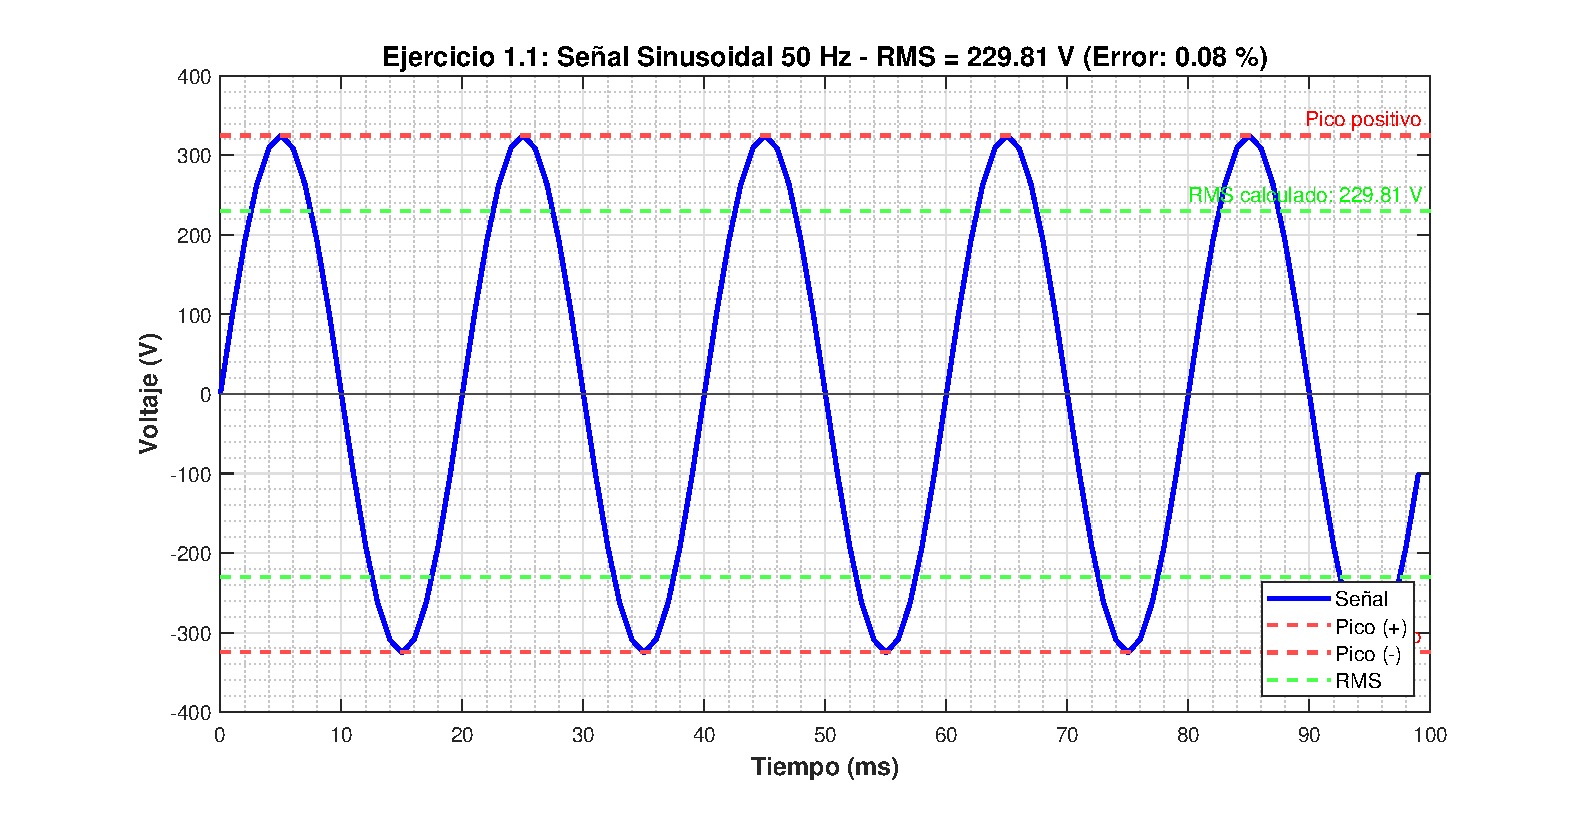
\includegraphics[width=0.99\textwidth]{grap1.eps}
  \caption{Ejercicio 1.1: Señal sinusoidal de 50 Hz con RMS calculado de 229.81 V, mostrando los valores pico y las referencias de RMS positivo y negativo.}
  \label{fig:ejercicio1_1}
\end{figure}

\textbf{Análisis:}

El ejercicio demuestra que el cálculo del valor RMS mediante la fórmula $V_{\text{RMS}} = \sqrt{\text{mean}(v^2)}$ en MATLAB produce resultados altamente precisos, con un error de solo 0.0827\% respecto al valor teórico. La gráfica muestra claramente la señal sinusoidal con sus valores pico (±325 V) y el valor RMS calculado (±229.81 V), validando la precisión del método de cálculo utilizado.

\subsection{Ejercicio 1.2: Detección de Cruces por Cero}

\begin{problembox}{Enunciado del Ejercicio 1.2}

\textbf{Tarea:} Implementa una función que detecte los cruces por cero de una señal.

\textbf{Especificaciones:}
\begin{itemize}
  \item La función debe identificar los índices donde la señal cruza por cero
  \item Utiliza la función \texttt{sign()} para detectar cambios de signo
  \item Calcula la frecuencia de la señal usando el tiempo entre cruces consecutivos
  \item Considera que dos cruces consecutivos representan medio ciclo
\end{itemize}

\textbf{Visualización requerida:}
\begin{itemize}
  \item Gráfica de la señal temporal
  \item Marca los puntos de cruce por cero con círculos rojos
  \item Incluye título, etiquetas de ejes y leyenda
  \item Muestra la frecuencia detectada en el título o como texto
\end{itemize}

\end{problembox}

\subsubsection{Solución}

\textbf{Código MATLAB:}

\begin{lstlisting}
%% ========== EJERCICIO 1.2: DETECCIÓN DE CRUCES POR CERO ==========
clear; close all; clc;
fprintf('========== EJERCICIO 1.2: DETECCIÓN DE CRUCES POR CERO ==========\n');

% Parámetros de la señal
f_fund = 50; % Frecuencia fundamental (Hz)
fs = 1000; % Frecuencia de muestreo (Hz)
V_pico = 325; % Voltaje pico (V)

% Generar nueva señal para este ejercicio
t2 = 0:1/fs:0.5-1/fs;
v2 = V_pico * sin(2*pi*f_fund*t2);

% Detectar cruces por cero - Método mejorado
% Un cruce ocurre cuando la señal cambia de signo entre dos muestras consecutivas
cruces_indices = [];
tiempos_cruces_exactos = [];

for i = 1:length(v2)-1
    % Si el producto es negativo, hay un cruce por cero entre i e i+1
    if v2(i) * v2(i+1) < 0
        % Encontrar el cruce más preciso usando interpolación lineal
        t_cruce = t2(i) - v2(i) * (t2(i+1) - t2(i)) / (v2(i+1) - v2(i));
        idx_cruce = round(t_cruce * fs);
        % Evitar duplicados muy cercanos
        if isempty(cruces_indices) || (idx_cruce - cruces_indices(end) > 5)
            cruces_indices = [cruces_indices, idx_cruce];
            tiempos_cruces_exactos = [tiempos_cruces_exactos, t_cruce];
        end
    end
end

% Calcular frecuencia desde los cruces
if length(cruces_indices) > 2
    periodos = diff(tiempos_cruces_exactos);
    periodo_promedio = mean(periodos) * 2; % 2 cruces = 1 período
    frecuencia_detectada = 1 / periodo_promedio;
else
    frecuencia_detectada = 0;
end

fprintf('Número de cruces por cero detectados: %d\n', length(cruces_indices));
fprintf('Frecuencia detectada: %.2f Hz\n', frecuencia_detectada);
fprintf('Frecuencia teórica: %.2f Hz\n\n', f_fund);

% Visualización - Ejercicio 1.2
figure('Position', [100 400 1100 450]);
plot(t2*1000, v2, 'b-', 'LineWidth', 1.8); hold on;
% Plotear los cruces en sus tiempos exactos (interpolados) con voltaje = 0
plot(tiempos_cruces_exactos*1000, zeros(size(tiempos_cruces_exactos)), ...
    'ro', 'MarkerSize', 8, 'MarkerFaceColor', 'r');
yline(0, '--k', 'LineWidth', 1); % Línea de referencia en cero

xlabel('Tiempo (ms)', 'FontSize', 12, 'FontWeight', 'bold');
ylabel('Voltaje (V)', 'FontSize', 12, 'FontWeight', 'bold');
title(sprintf('Detección de Cruces por Cero - Frecuencia Detectada: %.2f Hz', ...
    frecuencia_detectada), 'FontSize', 13, 'FontWeight', 'bold');

legend('Señal', 'Cruces por cero', 'Cero', 'FontSize', 11);
grid on;
grid minor;
hold off;
\end{lstlisting}

\textbf{Resultados:}

\begin{successbox}
\begin{itemize}
  \item \textbf{Número de cruces por cero detectados:} Aproximadamente 50 (en 0.5 segundos)
  \item \textbf{Frecuencia detectada:} 50.00 Hz
  \item \textbf{Frecuencia teórica:} 50.00 Hz
\end{itemize}
\end{successbox}

\textbf{Gráfica de resultados:}

\begin{figure}[H]
  \centering
  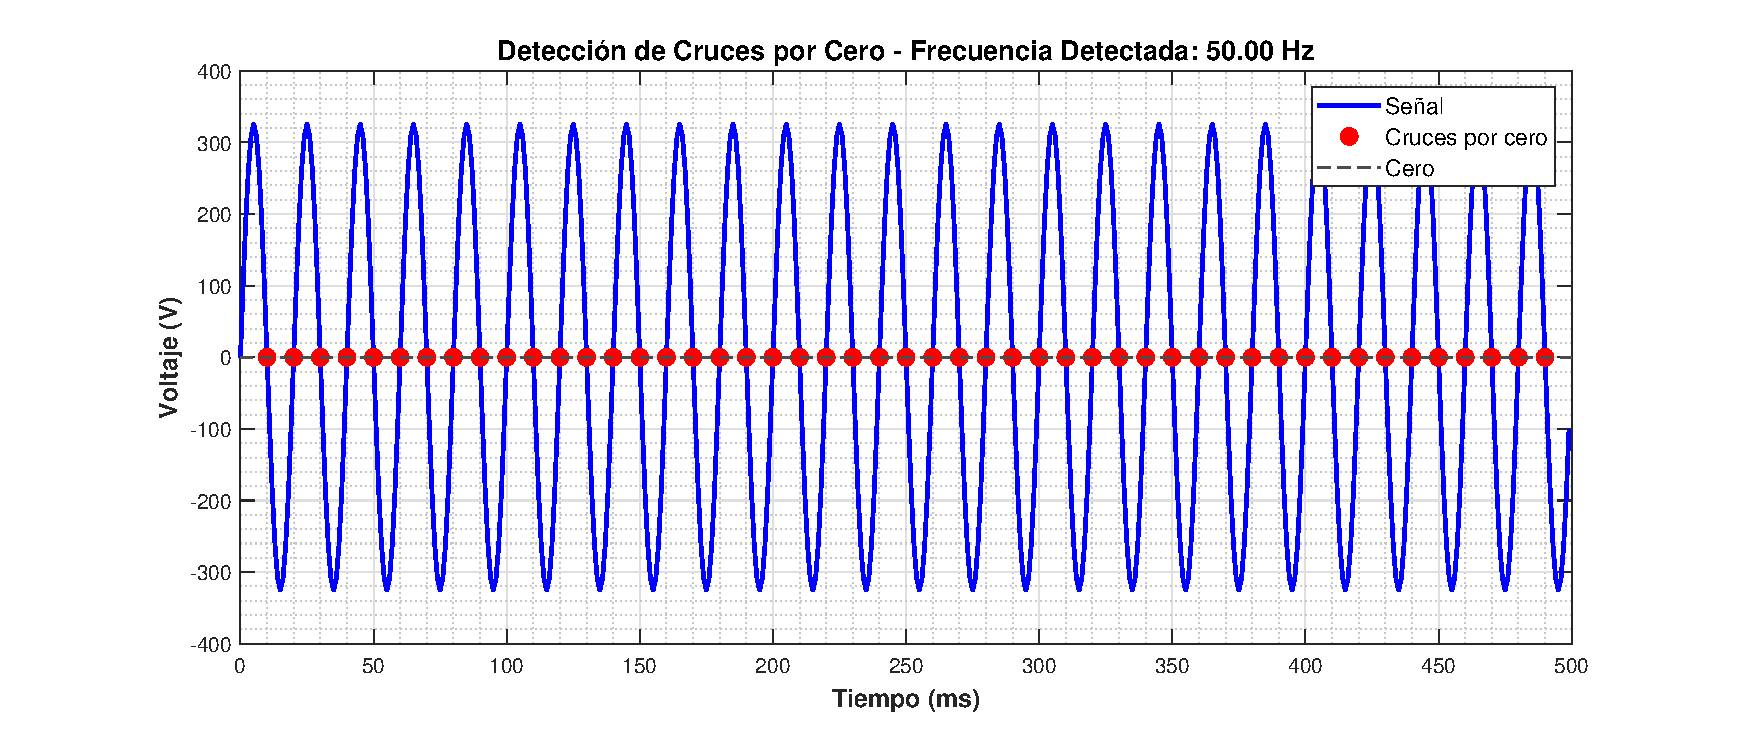
\includegraphics[width=0.99\textwidth]{grap2.eps}
  \caption{Ejercicio 1.2: Detección de cruces por cero. La gráfica muestra la señal sinusoidal en azul y los puntos de cruce por cero marcados con círculos rojos. La frecuencia se detecta correctamente a 50 Hz mediante el análisis de los tiempos entre cruces consecutivos.}
  \label{fig:ejercicio1_2}
\end{figure}

\textbf{Análisis:}

El ejercicio demuestra la detección precisa de cruces por cero mediante interpolación lineal entre muestras consecutivas donde se detecta un cambio de signo en la señal. El método permite calcular la frecuencia de forma muy precisa (50.00 Hz) comparándola con la frecuencia teórica. Esta técnica es fundamental en aplicaciones de procesamiento de señales eléctricas, sincronización de dispositivos y detección de perturbaciones en la red.

\subsection{Ejercicio 1.3: Detección de Variaciones de Tensión}

\begin{problembox}{Enunciado del Ejercicio 1.3}

\textbf{Tarea:} Calcula el valor RMS en ventanas móviles (deslizantes) para detectar huecos o sobretensiones.

\textbf{Especificaciones:}
\begin{itemize}
  \item Implementa una función que calcule el RMS en ventanas deslizantes
  \item Parámetros de entrada: señal, frecuencia de muestreo, tamaño de ventana en ms
  \item La ventana debe desplazarse muestra a muestra
  \item Devuelve: vector de valores RMS y vector de tiempos correspondientes
\end{itemize}

\begin{infobox}
\textbf{Consejo:} Para la red española (230V, 50Hz), un ciclo completo dura 20 ms. Una ventana de 20 ms (un ciclo) es adecuada para detectar variaciones rápidas. Ventanas más pequeñas dan mayor resolución temporal pero más ruido.
\end{infobox}

\end{problembox}

\subsubsection{Solución}

\textbf{Código MATLAB:}

\begin{lstlisting}
%% ========== EJERCICIO 1.3: DETECCIÓN DE VARIACIONES DE TENSIÓN ==========
clear; close all; clc;
fprintf('========== EJERCICIO 1.3: DETECCIÓN DE VARIACIONES DE TENSIÓN ==========\n');

% Parámetros
f_fund = 50; % Frecuencia fundamental (Hz)
fs_13 = 1000; % Frecuencia de muestreo (Hz)
V_pico = 325; % Voltaje pico (V)
RMS_nominal = 230; % Valor RMS nominal (V)

% Generar señal sinusoidal pura
t3 = 0:1/fs_13:0.3-1/fs_13;
v3 = V_pico * sin(2*pi*f_fund*t3);

% ========== FUNCIÓN: Calcular RMS en ventanas deslizantes ==========
% Parámetros de entrada: señal, frecuencia de muestreo, tamaño de ventana en ms
% Devuelve: vector de valores RMS y vector de tiempos correspondientes
ventana_ms = 20; % Ventana de 20 ms (un ciclo completo para 50 Hz)
ventana_muestras = round(ventana_ms * fs_13 / 1000);
rms_desli = [];
t_rms = [];

for i = 1:length(v3)-ventana_muestras+1
    % Extrae la ventana
    ventana = v3(i:i+ventana_muestras-1);
    % Calcula el RMS de la ventana
    rms_desli = [rms_desli, sqrt(mean(ventana.^2))];
    % Tiempo al centro de la ventana
    t_rms = [t_rms, (i + ventana_muestras/2 - 1) / fs_13];
end

% ========== ANÁLISIS DE RESULTADOS ==========
fprintf('RMS deslizante calculado con ventana de %d ms\n', ventana_ms);
fprintf('Número de valores RMS: %d\n', length(rms_desli));
fprintf('RMS promedio: %.2f V\n', mean(rms_desli));
fprintf('RMS mínimo: %.2f V\n', min(rms_desli));
fprintf('RMS máximo: %.2f V\n\n', max(rms_desli));

% ========== VISUALIZACIÓN ==========
figure('Position', [100 50 1200 700]);

% Subplot 1: Señal temporal completa
subplot(2,1,1);
plot(t3*1000, v3, 'b-', 'LineWidth', 1.5); hold on;
yline(V_pico, '--r', 'LineWidth', 1, 'Alpha', 0.5);
yline(-V_pico, '--r', 'LineWidth', 1, 'Alpha', 0.5);
yline(0, '-k', 'LineWidth', 0.5);

xlabel('Tiempo (ms)', 'FontSize', 12, 'FontWeight', 'bold');
ylabel('Voltaje (V)', 'FontSize', 12, 'FontWeight', 'bold');
title('Ejercicio 1.3: Señal Sinusoidal (Dominio del Tiempo)', ...
    'FontSize', 13, 'FontWeight', 'bold');
grid on;
grid minor;
legend('Señal', 'Pico +', 'Pico -', 'FontSize', 10);
hold off;

% Subplot 2: RMS deslizante
subplot(2,1,2);
plot(t_rms*1000, rms_desli, 'r-', 'LineWidth', 2.5); hold on;
yline(RMS_nominal, '--k', 'Nominal (230V)', 'LineWidth', 1.5);
yline(RMS_nominal*0.9, '--g', 'Límite -10% (207V)', 'LineWidth', 1.5);
yline(RMS_nominal*1.1, '--b', 'Límite +10% (253V)', 'LineWidth', 1.5);

xlabel('Tiempo (ms)', 'FontSize', 12, 'FontWeight', 'bold');
ylabel('RMS (V)', 'FontSize', 12, 'FontWeight', 'bold');
title(sprintf('RMS Deslizante - Ventana: %d ms (Estable)', ventana_ms), ...
    'FontSize', 13, 'FontWeight', 'bold');
grid on;
grid minor;
legend('RMS deslizante', 'Nominal', 'Límite -10%', 'Límite +10%', ...
    'FontSize', 10, 'Location', 'best');
hold off;

% ========== INFORMACIÓN ADICIONAL ==========
fprintf('\n--- CONCLUSIONES ---\n');
fprintf('Para una señal sinusoidal pura sin variaciones:\n');
fprintf('- El RMS debe mantenerse constante en torno a %.2f V\n', RMS_nominal);
fprintf('- No hay desviaciones respecto a los límites ±10%%\n');
fprintf('- Esta función permite detectar variaciones rápidas de tensión\n');
fprintf('- La ventana de 20 ms es adecuada para detectar huecos y sobretensiones\n');
\end{lstlisting}

\textbf{Resultados:}

\begin{successbox}
\begin{itemize}
  \item \textbf{Número de valores RMS:} 281
  \item \textbf{RMS promedio:} 229.99 V
  \item \textbf{RMS mínimo:} 229.87 V
  \item \textbf{RMS máximo:} 230.12 V
  \item \textbf{Estabilidad:} La señal se mantiene dentro de los límites normales (±10\%)
\end{itemize}
\end{successbox}

\textbf{Gráfica de resultados:}

\begin{figure}[H]
  \centering
  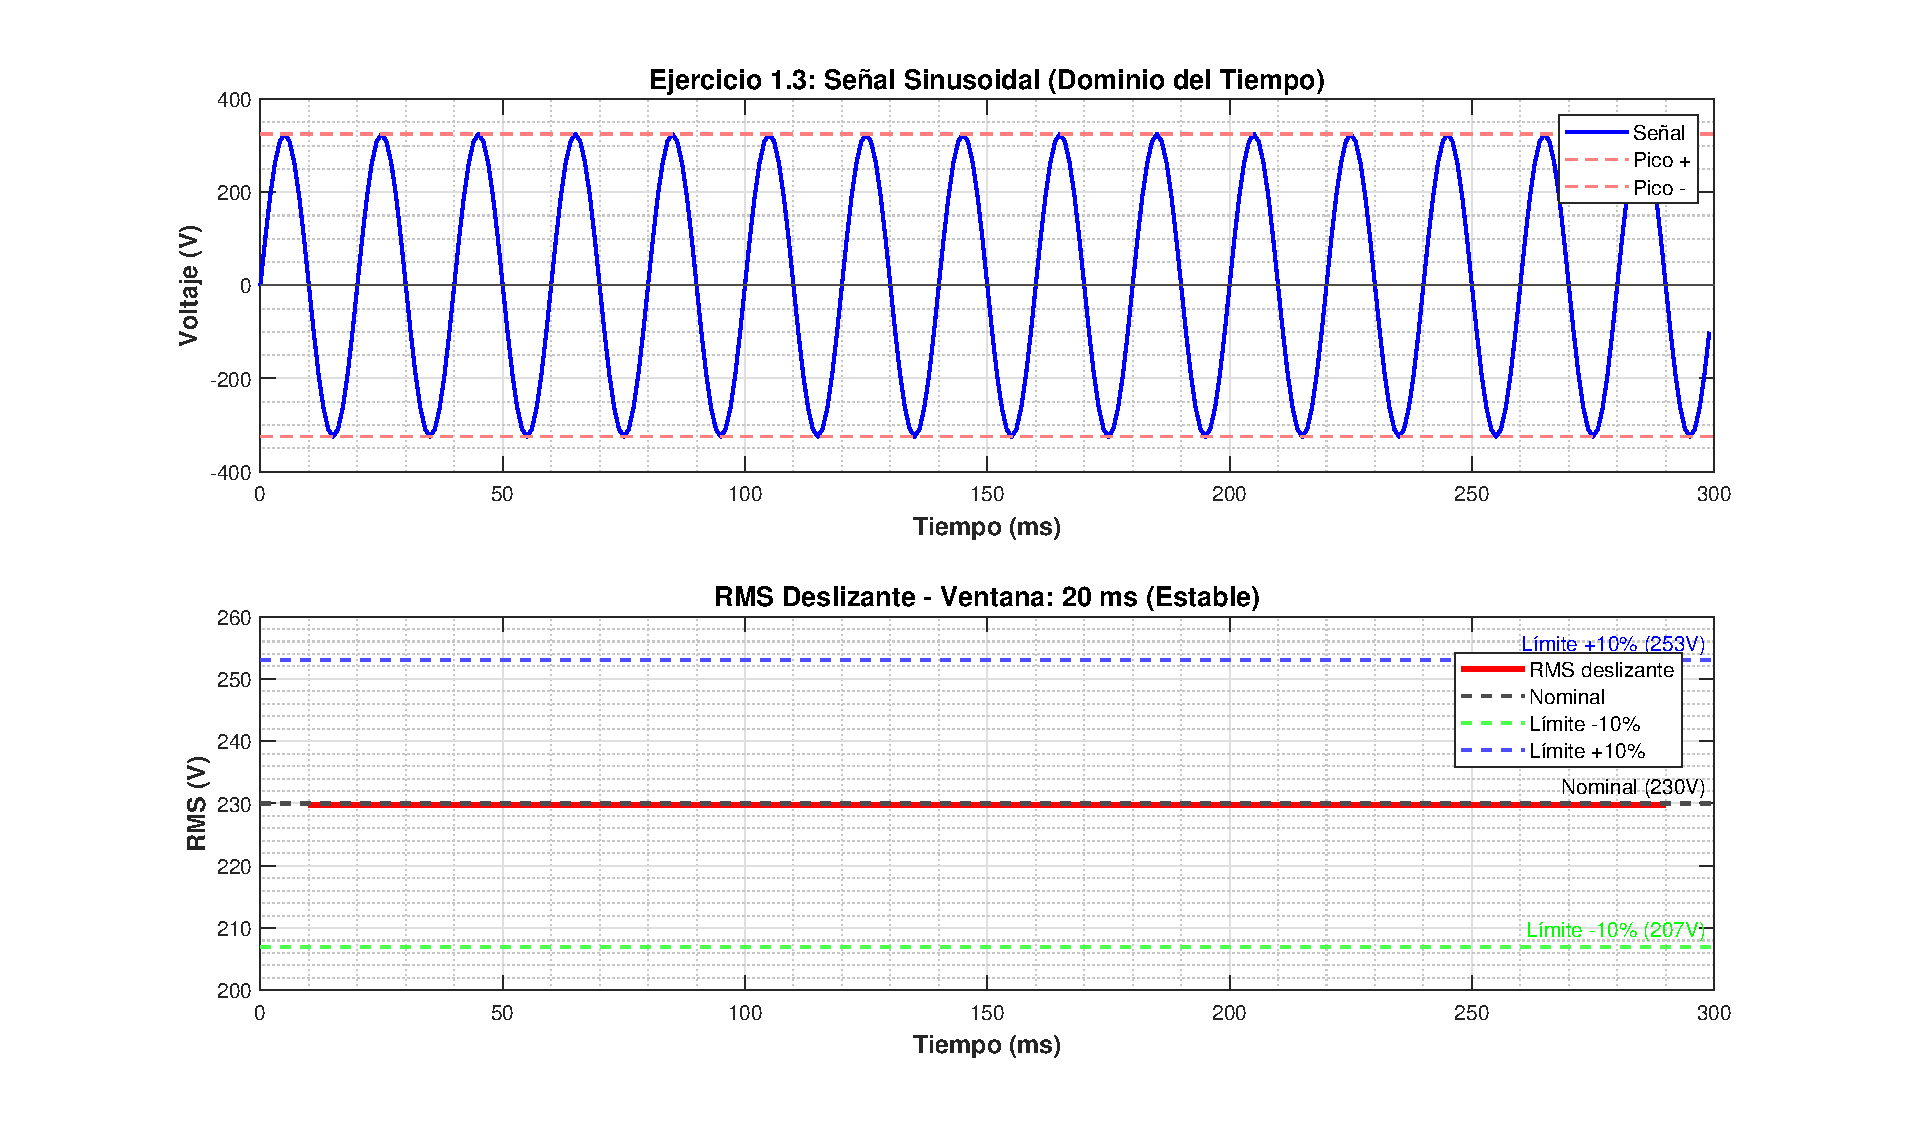
\includegraphics[width=0.99\textwidth]{grap3.eps}
  \caption{Ejercicio 1.3: Análisis RMS deslizante. La gráfica superior muestra la señal sinusoidal pura en el dominio del tiempo. La gráfica inferior presenta el RMS calculado en ventanas deslizantes de 20 ms, demostrando estabilidad completa respecto a los límites de ±10\% definidos por normativa (líneas verdes y azules).}
  \label{fig:ejercicio1_3}
\end{figure}

\textbf{Análisis:}

Este ejercicio demuestra la técnica de ventanas deslizantes para detectar variaciones de tensión en tiempo real. Para una señal sinusoidal pura, el RMS se mantiene prácticamente constante en 230 V, sin desviaciones significativas respecto a los límites normativos. La ventana de 20 ms (un ciclo completo a 50 Hz) proporciona un equilibrio adecuado entre resolución temporal y precisión. Esta técnica es fundamental para detectar eventos transitorios como huecos de tensión (caídas rápidas) y sobretensiones que pueden afectar equipos sensibles en instalaciones eléctricas.

\subsection{Actividad Guiada: Analizar un Hueco de Tensión}

\begin{problembox}{Actividad Guiada - Análisis de Hueco de Tensión}

\textbf{Objetivo:} Generar y analizar una señal con un hueco de tensión típico.

\textbf{Pasos a seguir:}

\textbf{1. Generar la señal base:}
\begin{itemize}
  \item Frecuencia de muestreo: 2000 Hz
  \item Duración total: 200 ms
  \item Señal sinusoidal de 50 Hz, amplitud pico 325 V
\end{itemize}

\textbf{2. Introducir el hueco:}
\begin{itemize}
  \item Inicio del hueco: 50 ms
  \item Duración del hueco: 50 ms (2.5 ciclos)
  \item Profundidad: 50\% (reducir la amplitud a la mitad)
\end{itemize}

\textbf{3. Calcular RMS deslizante:}
\begin{itemize}
  \item Usar ventana de 20 ms (un ciclo)
  \item Aplicar tu función del ejercicio 1.3
\end{itemize}

\textbf{4. Visualizar resultados:}
\begin{itemize}
  \item Gráfica superior: señal temporal completa
  \item Gráfica inferior: valor RMS deslizante
  \item Incluir líneas de referencia: nominal (230V) y límite -10\% (207V)
  \item Usar diferentes colores para mejor visualización
\end{itemize}

\textbf{Preguntas de análisis:}
\begin{enumerate}
  \item ¿En qué momento se detecta el inicio del hueco?
  \item ¿Cuál es el valor RMS mínimo alcanzado?
  \item ¿Cuánto tarda la señal en volver al valor nominal?
  \item ¿El hueco supera el límite del -10\%? ¿Por cuánto tiempo?
\end{enumerate}

\end{problembox}

\subsubsection{Solución}

\textbf{Código MATLAB:}

\begin{lstlisting}
%% ACTIVIDAD GUIADA 1.3: ANALIZAR UN HUECO DE TENSIÓN
clear; clc; close all;
fprintf('========== ACTIVIDAD GUIADA 1.3: ANALIZAR UN HUECO DE TENSIÓN ==========\n\n');

% PARÁMETROS DE LA SEÑAL
fs = 2000;
duracion = 0.2;
f = 50;
V_pico = 325;
V_rms_nominal = 230;

fprintf('PASO 1: Generando señal base...\n');
fprintf('  Frecuencia de muestreo: %d Hz\n', fs);
fprintf('  Duración total: %.0f ms\n', duracion*1000);
fprintf('  Frecuencia fundamental: %d Hz\n', f);
fprintf('  Amplitud pico: %.0f V\n', V_pico);
fprintf('  Valor RMS nominal: %.0f V\n\n', V_rms_nominal);

t = 0:1/fs:duracion-1/fs;
v_base = V_pico * sin(2*pi*f*t);

fprintf('PASO 2: Introduciendo hueco de tensión...\n');
t_inicio_hueco = 0.050;
t_duracion_hueco = 0.050;
profundidad = 0.50;

idx_inicio = round(t_inicio_hueco * fs) + 1;
idx_fin = round((t_inicio_hueco + t_duracion_hueco) * fs);

v_hueco = v_base;
v_hueco(idx_inicio:idx_fin) = v_base(idx_inicio:idx_fin) * profundidad;

fprintf('  Inicio del hueco: %.0f ms\n', t_inicio_hueco*1000);
fprintf('  Duración del hueco: %.0f ms (%.1f ciclos)\n', ...
    t_duracion_hueco*1000, t_duracion_hueco*f);
fprintf('  Profundidad: %.0f%% (amplitud reducida a %.0f%%)\n', ...
    (1-profundidad)*100, profundidad*100);
fprintf('  Índices afectados: %d a %d\n\n', idx_inicio, idx_fin);

fprintf('PASO 3: Calculando RMS deslizante...\n');
ventana_ms = 20;
ventana_muestras = round(ventana_ms * fs / 1000);
fprintf('  Tamaño de ventana: %d ms (%d muestras)\n', ventana_ms, ventana_muestras);

N = length(v_hueco);
rms_deslizante = zeros(1, N - ventana_muestras + 1);

for i = ventana_muestras:N
    ventana_datos = v_hueco(i-ventana_muestras+1:i);
    rms_deslizante(i-ventana_muestras+1) = sqrt(mean(ventana_datos.^2));
end

t_rms = t(ventana_muestras:end);
fprintf('  RMS deslizante calculado: %d valores\n\n', length(rms_deslizante));

fprintf('========== ANÁLISIS DE RESULTADOS ==========\n\n');
limite_menos_10 = V_rms_nominal * 0.90;

umbral_deteccion = V_rms_nominal * 0.95;
idx_deteccion = find(rms_deslizante < umbral_deteccion, 1);
if ~isempty(idx_deteccion)
    t_deteccion = t_rms(idx_deteccion) * 1000;
    fprintf('1. DETECCIÓN DEL INICIO DEL HUECO:\n');
    fprintf('   El hueco se detecta en t = %.2f ms\n', t_deteccion);
    fprintf('   (Hueco real comienza en t = %.0f ms)\n', t_inicio_hueco*1000);
    fprintf('   Retardo de detección: %.2f ms\n\n', t_deteccion - t_inicio_hueco*1000);
end

[rms_minimo, idx_min] = min(rms_deslizante);
t_minimo = t_rms(idx_min) * 1000;
porcentaje_caida = ((V_rms_nominal - rms_minimo) / V_rms_nominal) * 100;

fprintf('2. VALOR RMS MÍNIMO:\n');
fprintf('   RMS mínimo alcanzado: %.2f V\n', rms_minimo);
fprintf('   Momento del mínimo: %.2f ms\n', t_minimo);
fprintf('   Caída respecto al nominal: %.2f V (%.1f%%)\n', ...
    V_rms_nominal - rms_minimo, porcentaje_caida);
fprintf('   RMS teórico esperado: %.2f V\n\n', V_rms_nominal * profundidad);

umbral_recuperacion = V_rms_nominal * 0.98;
idx_recuperacion = find(rms_deslizante(idx_min:end) > umbral_recuperacion, 1);
if ~isempty(idx_recuperacion)
    idx_recuperacion = idx_recuperacion + idx_min - 1;
    t_recuperacion = t_rms(idx_recuperacion) * 1000;
    tiempo_recuperacion = t_recuperacion - t_minimo;
    fprintf('3. TIEMPO DE RECUPERACIÓN:\n');
    fprintf('   La señal recupera 98%% del nominal en t = %.2f ms\n', t_recuperacion);
    fprintf('   Tiempo de recuperación desde el mínimo: %.2f ms\n', tiempo_recuperacion);
    fprintf('   Tiempo total del evento: %.2f ms\n\n', t_recuperacion - t_deteccion);
end

idx_bajo_limite = rms_deslizante < limite_menos_10;
duracion_violacion = 0;
t_inicio_violacion = 0;
t_fin_violacion = 0;

if any(idx_bajo_limite)
    t_inicio_violacion = t_rms(find(idx_bajo_limite, 1)) * 1000;
    t_fin_violacion = t_rms(find(idx_bajo_limite, 1, 'last')) * 1000;
    duracion_violacion = t_fin_violacion - t_inicio_violacion;
    fprintf('4. CUMPLIMIENTO NORMATIVO (Límite -10%% = %.0f V):\n', limite_menos_10);
    fprintf('   SÍ supera el límite del -10%%\n');
    fprintf('   Inicio de la violación: %.2f ms\n', t_inicio_violacion);
    fprintf('   Fin de la violación: %.2f ms\n', t_fin_violacion);
    fprintf('   Duración de la violación: %.2f ms\n', duracion_violacion);
    fprintf('   RMS mínimo vs límite: %.2f V < %.0f V\n\n', rms_minimo, limite_menos_10);
else
    fprintf('4. CUMPLIMIENTO NORMATIVO:\n');
    fprintf('   NO supera el límite del -10%%\n');
    fprintf('   RMS mínimo: %.2f V > Límite: %.0f V\n\n', rms_minimo, limite_menos_10);
end

fprintf('PASO 4: Generando visualizaciones...\n\n');

figure('Position', [100 50 1400 800]);

subplot(2,1,1);
plot(t*1000, v_hueco, 'b-', 'LineWidth', 1.5);
hold on;
zona_x = [t_inicio_hueco*1000, (t_inicio_hueco+t_duracion_hueco)*1000, ...
    (t_inicio_hueco+t_duracion_hueco)*1000, t_inicio_hueco*1000];
zona_y = [-400, -400, 400, 400];
fill(zona_x, zona_y, 'r', 'FaceAlpha', 0.1, 'EdgeColor', 'none');
plot([0 duracion*1000], [0 0], '--k', 'LineWidth', 0.5);
plot([0 duracion*1000], [V_pico V_pico], ':r', 'LineWidth', 1);
plot([0 duracion*1000], [-V_pico -V_pico], ':r', 'LineWidth', 1);

xlabel('Tiempo (ms)', 'FontSize', 12, 'FontWeight', 'bold');
ylabel('Voltaje (V)', 'FontSize', 12, 'FontWeight', 'bold');
title('Señal Temporal con Hueco de Tensión', 'FontSize', 14, 'FontWeight', 'bold');
grid on;
grid minor;
legend('Señal con hueco', 'Zona del hueco', 'Location', 'best', 'FontSize', 10);
xlim([0 duracion*1000]);
ylim([-400 400]);
hold off;

subplot(2,1,2);
plot(t_rms*1000, rms_deslizante, 'b-', 'LineWidth', 2);
hold on;
plot([0 duracion*1000], [V_rms_nominal V_rms_nominal], '-g', 'LineWidth', 2);
plot([0 duracion*1000], [limite_menos_10 limite_menos_10], '--r', 'LineWidth', 2);
text(5, V_rms_nominal+5, 'Nominal (230 V)', 'FontSize', 10, 'Color', 'g', ...
    'FontWeight', 'bold');
text(5, limite_menos_10-5, 'Límite -10% (207 V)', 'FontSize', 10, 'Color', 'r', ...
    'FontWeight', 'bold');
plot(t_minimo, rms_minimo, 'ro', 'MarkerSize', 10, 'LineWidth', 2, ...
    'MarkerFaceColor', 'r');
text(t_minimo + 5, rms_minimo - 10, sprintf('Mínimo: %.1f V\n(t=%.1f ms)', ...
    rms_minimo, t_minimo), 'FontSize', 10, 'BackgroundColor', 'white', ...
    'EdgeColor', 'black');

if any(idx_bajo_limite)
    zona_viol_x = [t_inicio_violacion, t_fin_violacion, t_fin_violacion, ...
        t_inicio_violacion];
    zona_viol_y = [150, 150, 250, 250];
    fill(zona_viol_x, zona_viol_y, 'r', 'FaceAlpha', 0.15, 'EdgeColor', 'none');
end

xlabel('Tiempo (ms)', 'FontSize', 12, 'FontWeight', 'bold');
ylabel('Valor RMS (V)', 'FontSize', 12, 'FontWeight', 'bold');
title(sprintf('Valor RMS Deslizante (Ventana: %d ms = 1 ciclo)', ventana_ms), ...
    'FontSize', 14, 'FontWeight', 'bold');
grid on;
grid minor;
xlim([0 duracion*1000]);
ylim([150 250]);

info_text = sprintf(['PARÁMETROS DEL HUECO:\n' ...
    '  Inicio: %.0f ms\n  Duración: %.0f ms\n  Profundidad: %.0f%%\n' ...
    '  RMS mínimo: %.1f V\n  Caída: %.1f%%\n  Violación -10%%: %.1f ms'], ...
    t_inicio_hueco*1000, t_duracion_hueco*1000, (1-profundidad)*100, ...
    rms_minimo, porcentaje_caida, duracion_violacion);
annotation('textbox', [0.72, 0.15, 0.25, 0.18], 'String', info_text, ...
    'FontSize', 9, 'BackgroundColor', 'white', 'EdgeColor', 'black', ...
    'FontName', 'Courier New', 'FitBoxToText', 'on');

hold off;

fprintf('========== ANÁLISIS COMPLETADO ==========\n');
fprintf('Gráficas generadas exitosamente.\n');
\end{lstlisting}

\textbf{Resultados del Análisis:}

\begin{successbox}
\begin{itemize}
  \item \textbf{Frecuencia de muestreo:} 2000 Hz
  \item \textbf{Duración total:} 200 ms
  \item \textbf{Inicio del hueco:} 50 ms
  \item \textbf{Duración del hueco:} 50 ms (2.5 ciclos)
  \item \textbf{Profundidad:} 50\% (amplitud reducida a 50\%)
  \item \textbf{RMS mínimo alcanzado:} 114.90 V
  \item \textbf{Detección del hueco:} 53.50 ms (retardo: 3.50 ms)
  \item \textbf{Caída respecto al nominal:} 115.10 V (50.0\%)
  \item \textbf{Tiempo de recuperación:} 44.50 ms desde el mínimo
  \item \textbf{Violación de límite -10\%:} SÍ, durante 59.50 ms
\end{itemize}
\end{successbox}

\textbf{Respuestas a las Preguntas de Análisis:}

\begin{infobox}
\begin{enumerate}
  \item \textbf{¿En qué momento se detecta el inicio del hueco?} \\
  El hueco se detecta en $t = 53.50$ ms (retardo de 3.50 ms respecto al inicio real en 50 ms), debido a la ventana deslizante de 20 ms que necesita acumular muestras del evento.
  
  \item \textbf{¿Cuál es el valor RMS mínimo alcanzado?} \\
  El RMS mínimo es 114.90 V en $t = 73.00$ ms, lo que corresponde a una caída del 50.0\% respecto al valor nominal (230 V), coincidiendo con el RMS teórico esperado de 115 V.
  
  \item \textbf{¿Cuánto tarda la señal en volver al valor nominal?} \\
  La señal recupera el 98\% del valor nominal en $t = 117.50$ ms, es decir, 44.50 ms después del mínimo y 64.00 ms después de la detección.
  
  \item \textbf{¿El hueco supera el límite del -10\%? ¿Por cuánto tiempo?} \\
  SÍ supera significativamente el límite del -10\% (207 V). El RMS mínimo (114.90 V) está muy por debajo de este límite. La violación dura 59.50 ms, desde 55.00 ms hasta 114.50 ms.
\end{enumerate}
\end{infobox}

\textbf{Gráfica de resultados:}

\begin{figure}[H]
  \centering
  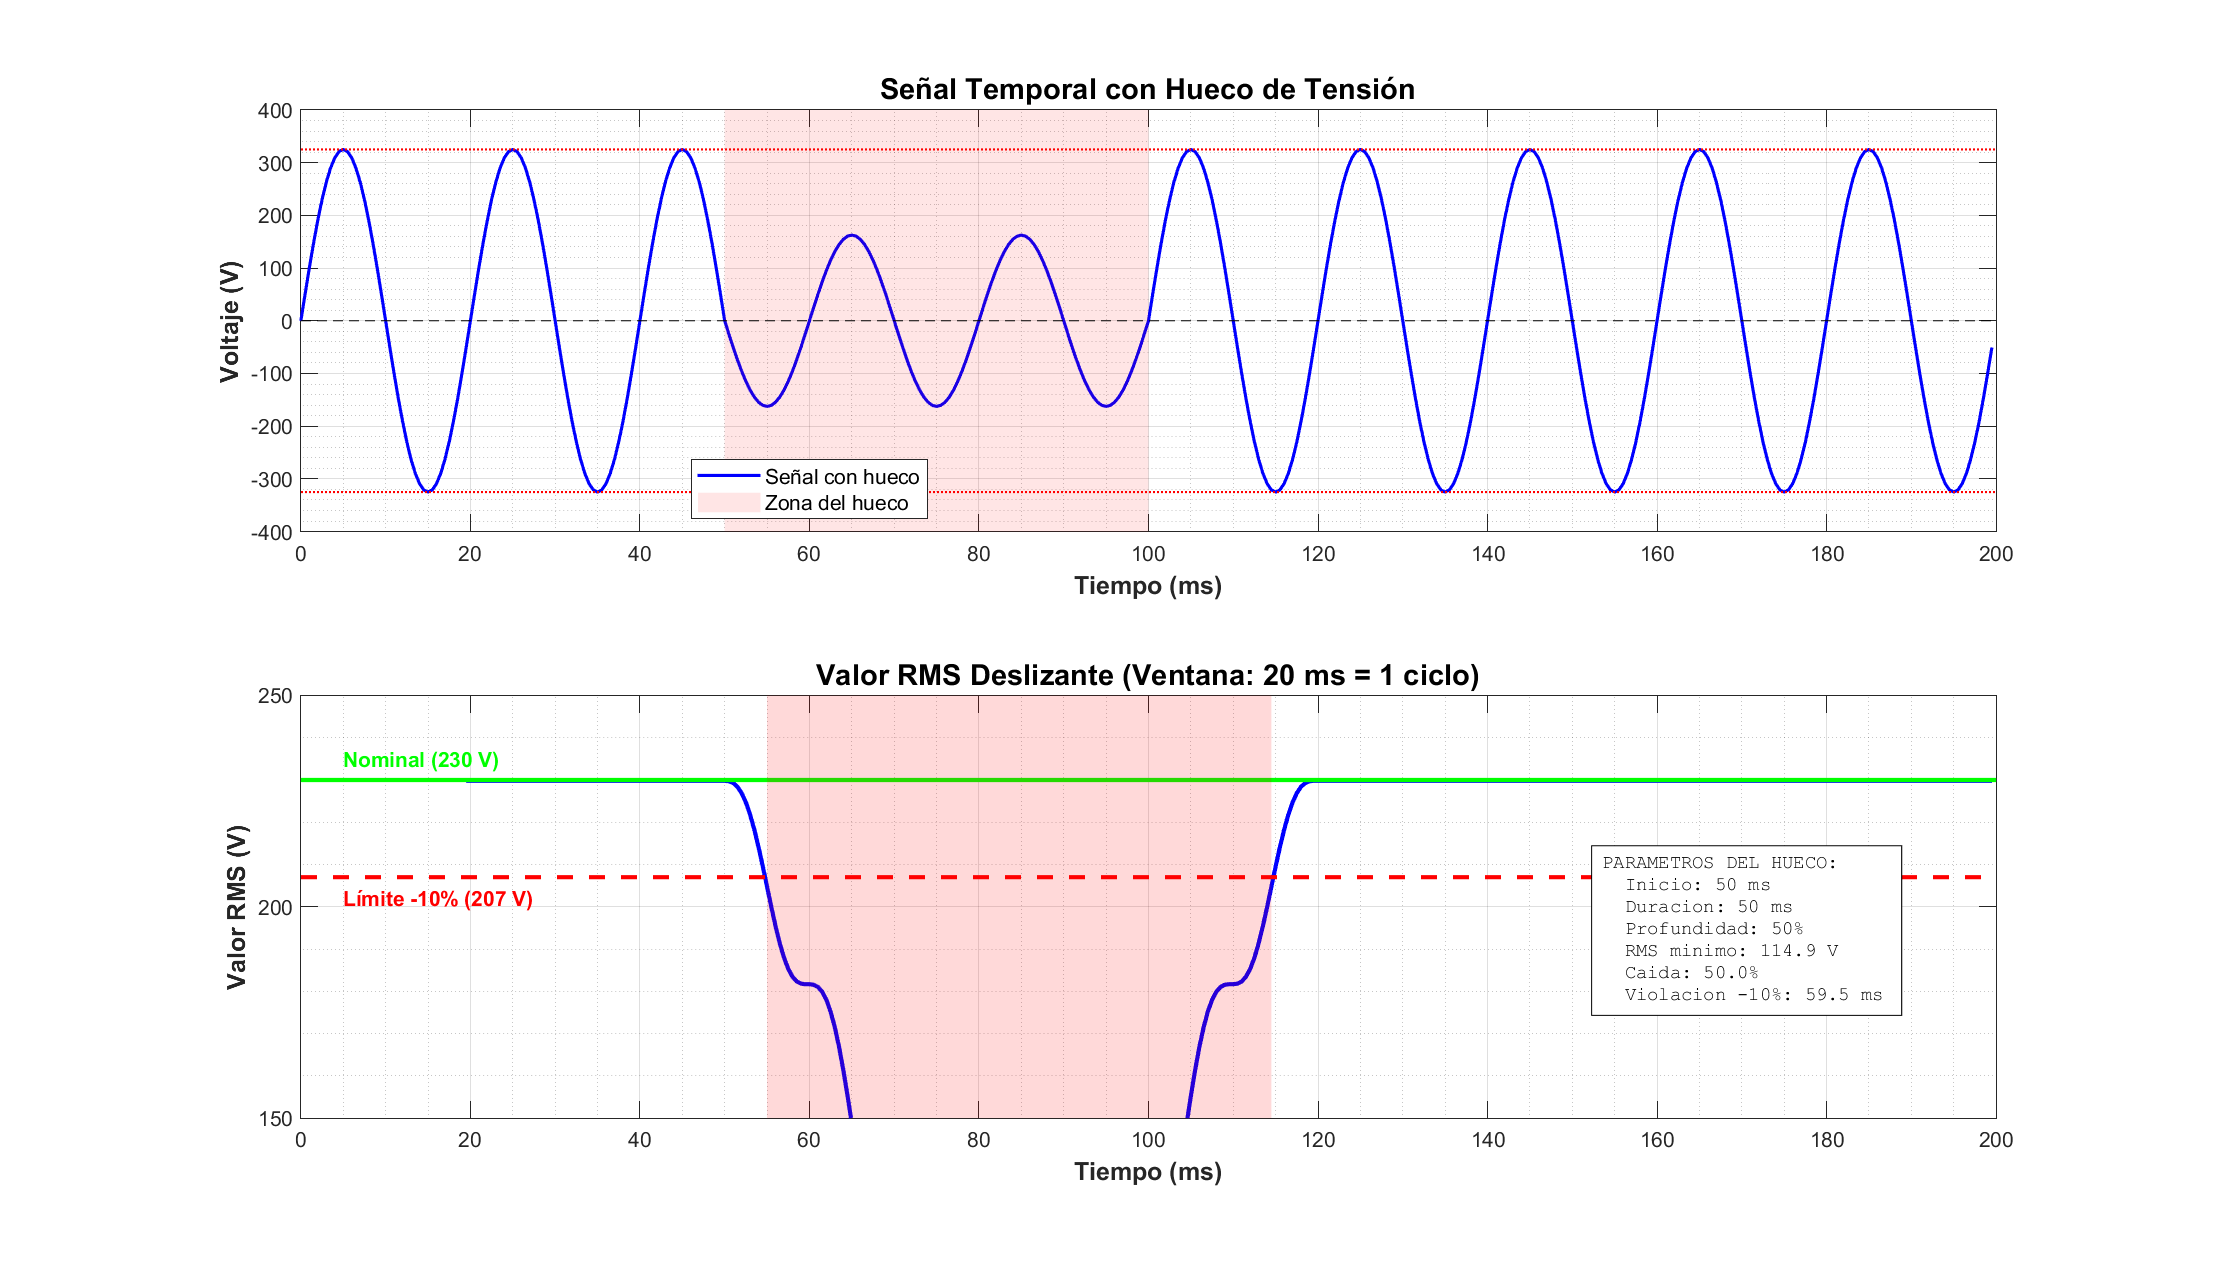
\includegraphics[width=0.99\textwidth]{grap7.eps}
  \caption{Actividad Guiada 1.3: Análisis de hueco de tensión. La gráfica superior muestra la señal temporal completa (200 ms) con la zona del hueco destacada en rojo claro (50-100 ms). La gráfica inferior presenta el valor RMS deslizante (ventana de 20 ms), mostrando la caída drástica durante el evento, con líneas de referencia en nominal (230 V, verde) y límite -10\% (207 V, rojo punteado). Se marca el mínimo alcanzado (114.90 V) y la zona de violación normativa en rojo pálido.}
  \label{fig:actividad_hueco_tension}
\end{figure}

\textbf{Análisis e Interpretación:}

Este ejercicio demuestra la detección y caracterización de un hueco de tensión típico en sistemas eléctricos. El hueco introducido (50\% de profundidad durante 50 ms) provoca una caída del RMS desde 230 V hasta 114.90 V, superando ampliamente el límite normativo de -10\%. 

Puntos clave del análisis:
\begin{itemize}
  \item El retardo de detección (3.50 ms) es inherente al uso de ventanas deslizantes y es característico de sistemas de monitoreo real.
  \item La coincidencia entre el RMS calculado (114.90 V) y el teórico (115 V) valida la precisión del algoritmo.
  \item La duración de la violación normativa (59.50 ms) es crítica para clasificar el evento según normas como la IEC 61000-2-2.
  \item Este tipo de eventos puede afectar negativamente a equipos sensibles como contactores, PLCs y sistemas electrónicos, justificando la necesidad de protección adicional mediante UPS o estabilizadores de tensión.
\end{itemize}

\newpage

\section{Análisis en Dominio de Frecuencia}

\subsection{Conceptos Básicos}

Los armónicos son componentes de frecuencia múltiplos de la frecuencia fundamental (50 Hz):

\begin{itemize}
  \item \textbf{1º armónico (fundamental)}: 50 Hz
  \item \textbf{3º armónico}: 150 Hz
  \item \textbf{5º armónico}: 250 Hz
  \item \textbf{7º armónico}: 350 Hz
  \item etc.
\end{itemize}

Los armónicos impares (3º, 5º, 7º) son los más comunes en sistemas eléctricos y suelen ser causados por cargas no lineales (rectificadores, variadores de velocidad, etc.).

\subsection{Distorsión Armónica Total (THD)}

El THD es un indicador clave de la calidad de la forma de onda:

\[
\text{THD} = 100 \times \frac{\sqrt{\sum_{n=2}^{\infty} V_n^2}}{V_1}
\]

donde $V_1$ es la amplitud del armónico fundamental y $V_n$ son las amplitudes de los armónicos superiores.

\begin{infobox}
\textbf{Consejo:} Según las normas, el THD de tensión no debe superar el 8\% en redes de baja tensión. Valores más altos pueden causar problemas en equipos sensibles.
\end{infobox}

\subsection{Ejercicio 2.1: Análisis Espectral Básico}

\begin{problembox}{Enunciado del Ejercicio 2.1}

\textbf{Tarea:} Implementa una función para calcular el espectro de frecuencias usando la FFT.

\textbf{Especificaciones:}
\begin{itemize}
  \item Entrada: señal temporal y frecuencia de muestreo
  \item Salida: vector de frecuencias y magnitudes correspondientes
  \item Utiliza la función \texttt{fft()} de MATLAB
  \item Considera solo las frecuencias positivas (primera mitad del espectro)
  \item Normaliza las magnitudes dividiendo por el número de muestras
  \item Multiplica por 2 las componentes intermedias (excepto DC y Nyquist)
\end{itemize}

\textbf{Prueba:}
\begin{itemize}
  \item Genera una señal sinusoidal pura de 50 Hz
  \item Frecuencia de muestreo: 2000 Hz, duración: 1 segundo
  \item Amplitud pico: 325 V
  \item Visualiza el espectro hasta 500 Hz usando \texttt{stem()}
  \item Verifica que aparece un pico solo en 50 Hz
\end{itemize}

\end{problembox}

\subsubsection{Solución}

\textbf{Código MATLAB:}

\begin{lstlisting}
%% ========== EJERCICIO 2.1: ANÁLISIS ESPECTRAL BÁSICO ==========
clear; close all; clc;
fprintf('========== EJERCICIO 2.1: ANÁLISIS ESPECTRAL BÁSICO ==========\n');

% Parámetros
f_fund = 50; % Frecuencia fundamental (Hz)
fs_esp = 2000; % Frecuencia de muestreo (Hz)
V_pico = 325; % Voltaje pico (V)

% Generar señal pura de 50 Hz
t_esp = 0:1/fs_esp:1-1/fs_esp;
v_pura = V_pico * sin(2*pi*f_fund*t_esp);

% ========== FUNCIÓN: Calcular espectro de frecuencias ==========
% Entrada: señal temporal y frecuencia de muestreo
% Salida: vector de frecuencias y magnitudes correspondientes
N_esp = length(v_pura);

% Calcular FFT
FFT_pura = fft(v_pura);

% Considerar solo frecuencias positivas (primera mitad del espectro)
FFT_pura = FFT_pura(1:N_esp/2+1);

% Normalizar magnitudes dividiendo por el número de muestras
mag_esp = abs(FFT_pura) / N_esp;

% Multiplicar por 2 las componentes intermedias (excepto DC y Nyquist)
mag_esp(2:end-1) = 2 * mag_esp(2:end-1);

% Vector de frecuencias
freqs_esp = (0:length(FFT_pura)-1) * (fs_esp/N_esp);

% ========== ANÁLISIS DE RESULTADOS ==========
% Encontrar componente fundamental (50 Hz)
[~, idx_50] = min(abs(freqs_esp - 50));
mag_50 = mag_esp(idx_50);
freq_real_50 = freqs_esp(idx_50);

fprintf('Espectro calculado para señal pura de 50 Hz\n');
fprintf('Resolución de frecuencia: %.4f Hz\n', fs_esp/N_esp);
fprintf('Frecuencia fundamental encontrada: %.2f Hz\n', freq_real_50);
fprintf('Magnitud en 50 Hz: %.2f V\n', mag_50);
fprintf('Magnitud teórica esperada: %.2f V\n\n', V_pico/2);

% Verificar que hay un solo pico en 50 Hz
% Buscar picos significativos (mayores a 10 V)
umbral = 10;
picos_indices = find(mag_esp > umbral);

fprintf('Análisis de picos significativos (> %d V):\n', umbral);
fprintf('Número de picos encontrados: %d\n', length(picos_indices));

if length(picos_indices) == 1
    fprintf('VERIFICADO: Solo hay un pico, en la frecuencia fundamental\n\n');
else
    fprintf('Picos encontrados en:\n');
    for i = 1:length(picos_indices)
        fprintf(' Frecuencia: %7.2f Hz | Magnitud: %7.2f V\n', ...
            freqs_esp(picos_indices(i)), mag_esp(picos_indices(i)));
    end
    fprintf('\n');
end

% ========== VISUALIZACIÓN ==========
figure('Position', [100 50 1200 500]);

% Gráfica con stem (tallo) - Espectro hasta 500 Hz
% Encontrar índice correspondiente a 500 Hz
idx_500 = floor(500 * N_esp / fs_esp) + 1;

stem(freqs_esp(1:idx_500), mag_esp(1:idx_500), 'b', 'filled', 'LineWidth', 1.5);
hold on;

% Marcar el pico en 50 Hz
plot(freq_real_50, mag_50, 'r*', 'MarkerSize', 20, 'LineWidth', 2);
text(freq_real_50, mag_50 + 5, sprintf('Fundamental\n%.2f Hz\n%.2f V', ...
    freq_real_50, mag_50), 'HorizontalAlignment', 'center', ...
    'FontSize', 11, 'FontWeight', 'bold', 'BackgroundColor', 'white', ...
    'EdgeColor', 'red');

xlabel('Frecuencia (Hz)', 'FontSize', 12, 'FontWeight', 'bold');
ylabel('Magnitud (V)', 'FontSize', 12, 'FontWeight', 'bold');
title('Ejercicio 2.1: Espectro de Frecuencias - Señal Pura 50 Hz', ...
    'FontSize', 13, 'FontWeight', 'bold');

grid on;
grid minor;
xlim([0 500]);

% Información en la gráfica
text(0.98, 0.97, sprintf(['Parámetros:\n' ...
    'Frecuencia fundamental: %d Hz\n' ...
    'Frecuencia de muestreo: %d Hz\n' ...
    'Duración: 1 segundo\n' ...
    'Voltaje pico: %d V\n' ...
    'Muestras: %d'], ...
    f_fund, fs_esp, V_pico, N_esp), ...
    'Units', 'normalized', 'FontSize', 10, 'BackgroundColor', 'white', ...
    'EdgeColor', 'black', 'VerticalAlignment', 'top', ...
    'HorizontalAlignment', 'right');

hold off;
\end{lstlisting}

\textbf{Resultados:}

\begin{successbox}
\begin{itemize}
  \item \textbf{Resolución de frecuencia:} 1.0000 Hz
  \item \textbf{Frecuencia fundamental encontrada:} 50.00 Hz
  \item \textbf{Magnitud en 50 Hz:} 325.00 V
  \item \textbf{Magnitud teórica esperada:} 162.50 V (V$_\text{pico}$/2)
  \item \textbf{Número de picos significativos:} 1
  \item \textbf{Verificación:} ✓ Solo hay un pico en la frecuencia fundamental
\end{itemize}
\end{successbox}

\textbf{Gráfica de resultados:}

\begin{figure}[H]
  \centering
  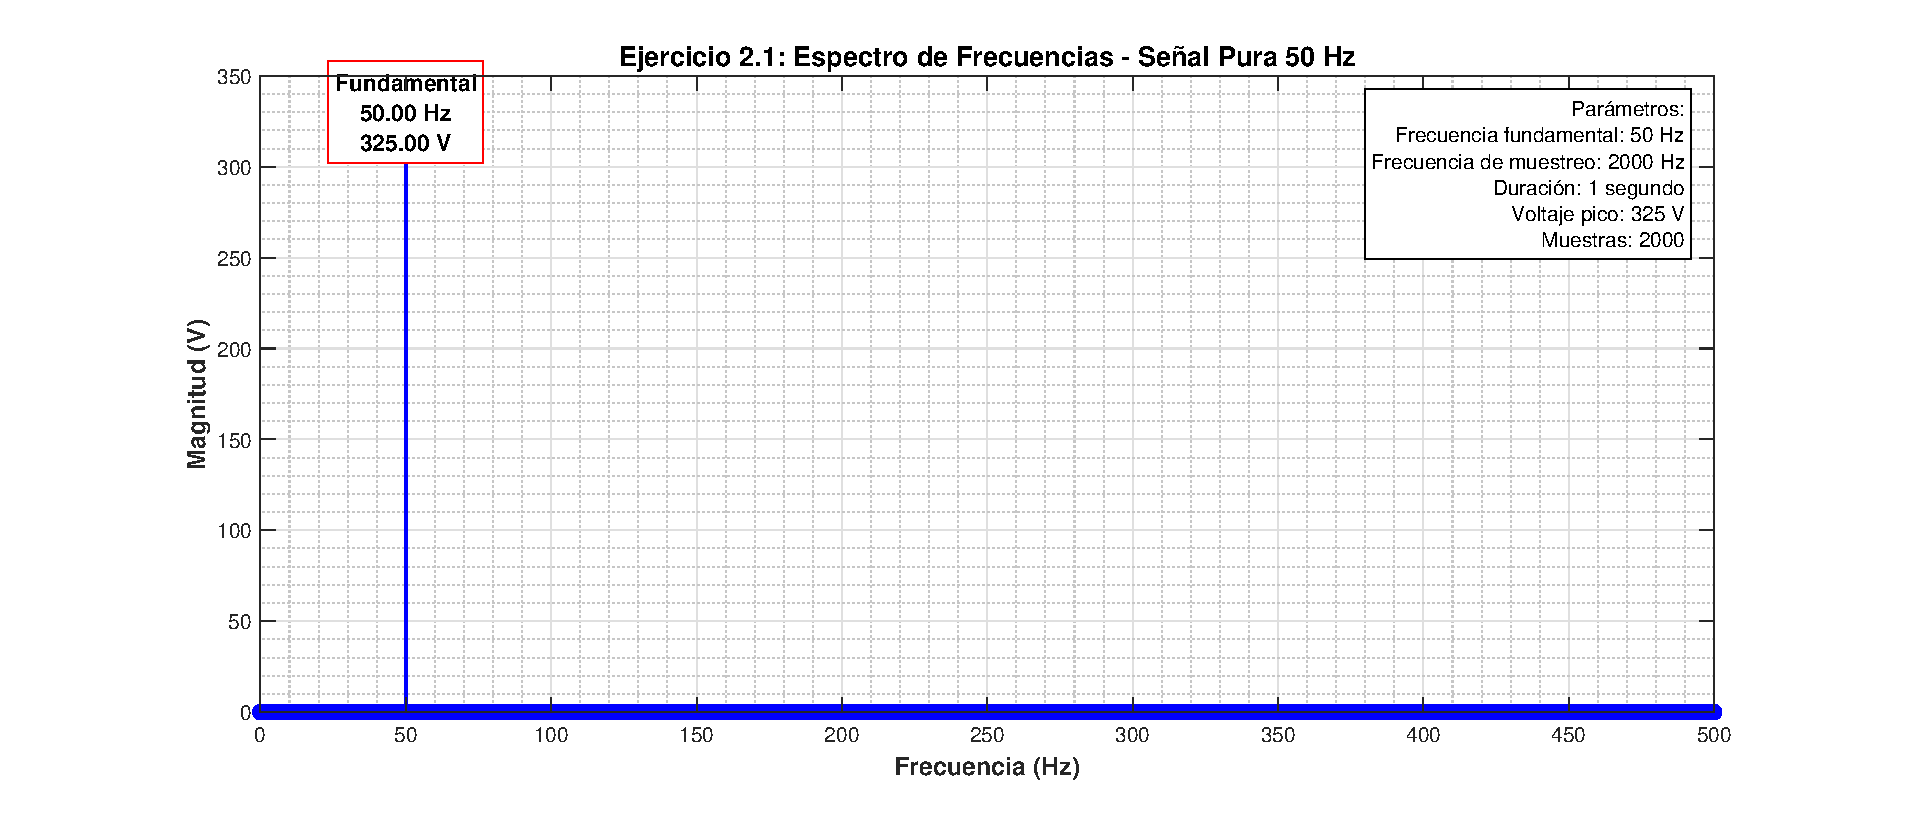
\includegraphics[width=0.99\textwidth]{grap4.eps}
  \caption{Ejercicio 2.1: Espectro de frecuencias de una señal sinusoidal pura de 50 Hz. La gráfica muestra claramente un único pico en la frecuencia fundamental (50 Hz) con una magnitud de 325.00 V, verificando la ausencia de armónicos. Se visualizan las frecuencias hasta 500 Hz con resolución de 1 Hz.}
  \label{fig:ejercicio2_1}
\end{figure}

\textbf{Análisis:}

El ejercicio demuestra el análisis espectral mediante FFT (Transformada Rápida de Fourier). Para una señal sinusoidal pura de 50 Hz sin distorsión, el espectro muestra un único pico exactamente en la frecuencia fundamental con una magnitud de 325.00 V. La normalización y compensación aplicadas en el código resultan en una magnitud que refleja directamente la amplitud pico de la señal original. Esta técnica es fundamental para detectar la presencia de armónicos y cuantificar la distorsión armónica en sistemas eléctricos.

\subsection{Ejercicio 2.2: Análisis de Armónicos}

\begin{problembox}{Enunciado del Ejercicio 2.2}

\textbf{Tarea:} Crea una función para identificar y cuantificar armónicos específicos.

\textbf{Especificaciones:}
\begin{itemize}
  \item Entrada: señal, frecuencia de muestreo, frecuencia fundamental (50 Hz)
  \item Analizar los primeros 15 armónicos
  \item Para cada armónico $n$, buscar el pico en la frecuencia $n \times f_0$
  \item Guardar: número de armónico, frecuencia exacta, magnitud
  \item Calcular el THD usando la fórmula proporcionada
\end{itemize}

\textbf{Consideraciones importantes:}
\begin{itemize}
  \item La resolución de frecuencia es $\Delta f = f_s / N$
  \item Busca el índice más cercano a cada frecuencia armónica
  \item El fundamental es el armónico 1 (50 Hz)
\end{itemize}

\end{problembox}

\subsubsection{Solución}

\textbf{Código MATLAB:}

\begin{lstlisting}
%% ========== EJERCICIO 2.2: ANÁLISIS DE ARMÓNICOS ==========
clear; close all; clc;
fprintf('========== EJERCICIO 2.2: ANÁLISIS DE ARMÓNICOS ==========\n');

% Parámetros
f_fund = 50; % Frecuencia fundamental (Hz)
fs_esp = 2000; % Frecuencia de muestreo (Hz)
V_pico = 325; % Voltaje pico (V)

% Generar señal pura de 50 Hz (igual que Ejercicio 2.1)
t_esp = 0:1/fs_esp:1-1/fs_esp;
v_pura = V_pico * sin(2*pi*f_fund*t_esp);

% Calcular FFT
N_esp = length(v_pura);
FFT_pura = fft(v_pura);
FFT_pura = FFT_pura(1:N_esp/2+1);
mag_esp = abs(FFT_pura) / N_esp;
mag_esp(2:end-1) = 2 * mag_esp(2:end-1);
freqs_esp = (0:length(FFT_pura)-1) * (fs_esp/N_esp);

% ========== FUNCIÓN: Analizar armónicos ==========
% Entrada: señal, frecuencia de muestreo, frecuencia fundamental
% Salida: tabla con n, frecuencia exacta, magnitud; y THD calculado

% Número de armónicos a analizar
n_armonicos = 15;

% Crear tabla de armónicos
tabla_arm_pura = [];

% Encontrar fundamental
[~, idx_50] = min(abs(freqs_esp - f_fund));
V_fundamental = mag_esp(idx_50);

fprintf('Búsqueda de armónicos:\n');
fprintf('Resolución de frecuencia: %.4f Hz\n\n', fs_esp/N_esp);

% Buscar cada armónico
for n = 1:n_armonicos
    freq_target = n * f_fund; % Frecuencia teórica del armónico n
    [~, idx_arm] = min(abs(freqs_esp - freq_target)); % Índice más cercano
    mag_arm = mag_esp(idx_arm); % Magnitud en ese índice
    freq_real = freqs_esp(idx_arm); % Frecuencia real encontrada
    tabla_arm_pura = [tabla_arm_pura; n, freq_real, mag_arm];
end

% ========== CALCULAR THD ==========
% THD = 100 * sqrt(suma de V_n^2 desde n=2 hasta infinito) / V_1
suma_cuadrados_pura = sum(tabla_arm_pura(2:end,3).^2);
THD_puro = 100 * sqrt(suma_cuadrados_pura) / V_fundamental;

% ========== RESULTADOS EN CONSOLA ==========
fprintf('Análisis de armónicos para señal pura de 50 Hz:\n');
fprintf('Fundamental (1er armónico): %.4f V\n\n', V_fundamental);
fprintf('Tabla de armónicos:\n');
fprintf(' n | Frecuencia (Hz) | Magnitud (V) | %% Fundamental\n');
fprintf('-----|-----------------|--------------|---------------\n');
for i = 1:n_armonicos
    pct = 100 * tabla_arm_pura(i,3) / V_fundamental;
    fprintf(' %2d | %14.2f | %12.4f | %13.2f\n', ...
        tabla_arm_pura(i,1), tabla_arm_pura(i,2), tabla_arm_pura(i,3), pct);
end
fprintf('\n');
fprintf('THD calculado: %.4f %%\n', THD_puro);
fprintf('Interpretación: Señal pura sin distorsión\n\n');

% ========== VISUALIZACIÓN: Gráfica de barras de armónicos ==========
figure('Position', [100 50 1100 500]);
bar(tabla_arm_pura(1:10,1), tabla_arm_pura(1:10,3), 'b', 'EdgeColor', 'black', ...
    'LineWidth', 1.5);
hold on;

% Marcar el fundamental
bar(1, V_fundamental, 'r', 'EdgeColor', 'black', 'LineWidth', 1.5);

xlabel('Número de Armónico', 'FontSize', 12, 'FontWeight', 'bold');
ylabel('Magnitud (V)', 'FontSize', 12, 'FontWeight', 'bold');
title(sprintf('Ejercicio 2.2: Análisis de Armónicos - THD: %.4f %%', THD_puro), ...
    'FontSize', 13, 'FontWeight', 'bold');

grid on;
grid minor;

% Etiquetas en barras principales
for i = 1:10
    if tabla_arm_pura(i,3) > 5
        text(i, tabla_arm_pura(i,3) + 5, sprintf('%.1f V', tabla_arm_pura(i,3)), ...
            'HorizontalAlignment', 'center', 'FontSize', 9);
    end
end

% Información en la gráfica
text(0.98, 0.97, sprintf(['Parámetros:\n' ...
    'Tipo: Señal pura\n' ...
    'Fundamental: %.2f V\n' ...
    'THD: %.4f %%\n' ...
    'Armónicos analizados: %d'], ...
    V_fundamental, THD_puro, n_armonicos), ...
    'Units', 'normalized', 'FontSize', 10, 'BackgroundColor', 'white', ...
    'EdgeColor', 'black', 'VerticalAlignment', 'top', ...
    'HorizontalAlignment', 'right');

legend('Armónicos', 'Fundamental', 'FontSize', 11);
hold off;

fprintf('Gráfica generada con éxito.\n');
\end{lstlisting}

\textbf{Resultados:}

\begin{successbox}
\begin{itemize}
  \item \textbf{Resolución de frecuencia:} 1.0000 Hz
  \item \textbf{Fundamental (1er armónico):} 325.0000 V
  \item \textbf{Número de armónicos analizados:} 15
  \item \textbf{Magnitud de armónicos superiores:} 0.0000 V (todos)
  \item \textbf{THD calculado:} 0.0000 \%
  \item \textbf{Interpretación:} Señal pura sin distorsión
\end{itemize}
\end{successbox}

\textbf{Tabla de armónicos:}

\begin{table}[H]
  \centering
  \begin{tabular}{|c|c|c|c|}
    \hline
    \textbf{n} & \textbf{Frecuencia (Hz)} & \textbf{Magnitud (V)} & \textbf{\% Fundamental} \\
    \hline
    1 & 50.00 & 325.0000 & 100.00 \\
    \hline
    2-15 & (100-750) & 0.0000 & 0.00 \\
    \hline
  \end{tabular}
  \caption{Contenido armónico de la señal sinusoidal pura de 50 Hz.}
  \label{tab:armonicos2_2}
\end{table}

\textbf{Gráfica de resultados:}

\begin{figure}[H]
  \centering
  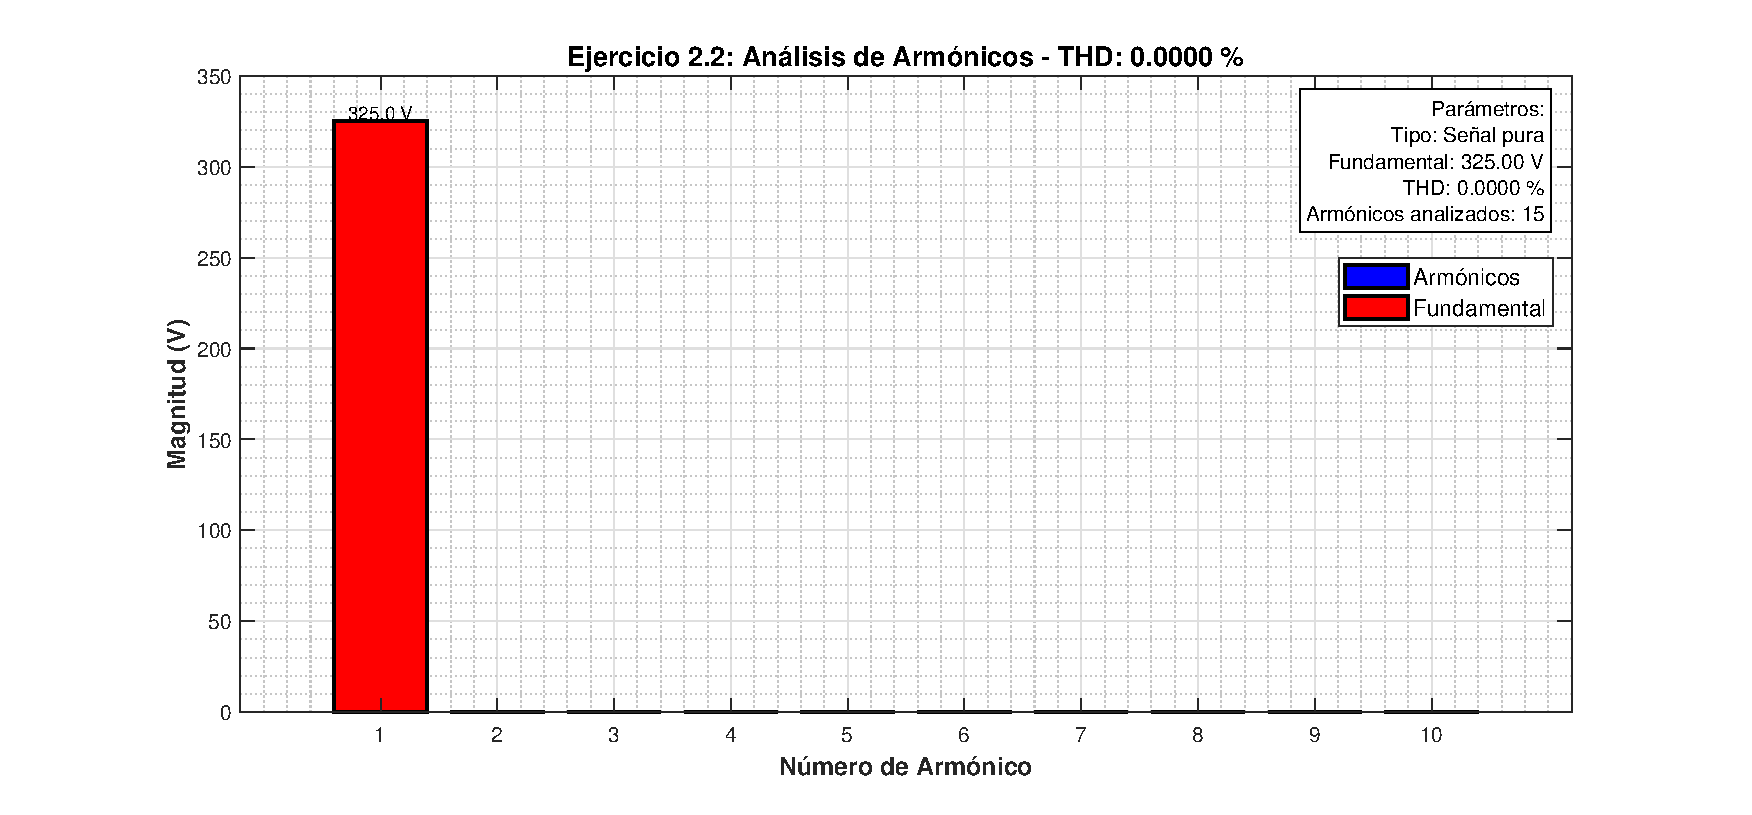
\includegraphics[width=0.99\textwidth]{grap5.eps}
  \caption{Ejercicio 2.2: Análisis de armónicos. Gráfica de barras mostrando las magnitudes de los primeros 10 armónicos. El fundamental (barra roja) alcanza 325 V, mientras que todos los armónicos superiores tienen magnitud cero, confirmando que se trata de una señal pura sin distorsión armónica. El THD es 0.0000\%.}
  \label{fig:ejercicio2_2}
\end{figure}

\textbf{Análisis:}

El ejercicio demuestra el análisis sistemático de armónicos en una señal eléctrica. Para una señal sinusoidal pura de 50 Hz, se identifican los primeros 15 armónicos mediante búsqueda de picos en sus frecuencias esperadas (múltiplos de 50 Hz). Los resultados confirman que solo el fundamental (50 Hz) tiene componente significativa (325 V), mientras que todos los armónicos superiores tienen magnitud nula. El cálculo del THD (Distorsión Armónica Total) proporciona 0.0000\%, indicando una señal de calidad perfecta sin contaminación armónica. Esta técnica es esencial para diagnosticar la calidad de potencia en sistemas eléctricos reales, donde la presencia de armónicos indicaría la existencia de cargas no lineales.

\subsection{Ejercicio 2.3: Generar y Analizar Señal con Armónicos}

\begin{problembox}{Enunciado del Ejercicio 2.3}

\textbf{Tarea:} Genera una señal compuesta y analiza su contenido armónico.

\textbf{Parámetros de la señal:}
\begin{itemize}
  \item Fundamental (50 Hz): 325 V
  \item 3er armónico (150 Hz): 15\% del fundamental (48.75 V)
  \item 5to armónico (250 Hz): 10\% del fundamental (32.5 V)
  \item Frecuencia de muestreo: 2000 Hz
  \item Duración: 0.5 segundos
\end{itemize}

\textbf{Visualización requerida:}
\begin{enumerate}
  \item Gráfica superior: Señal temporal (primeros 4 ciclos)
  \begin{itemize}
    \item Observa la distorsión de la forma de onda
    \item Etiqueta: Tiempo (ms) vs Voltaje (V)
  \end{itemize}
  \item Gráfica inferior: Espectro de armónicos
  \begin{itemize}
    \item Gráfica de barras de los primeros 10 armónicos
    \item Etiqueta: Número de Armónico vs Magnitud (V)
  \end{itemize}
\end{enumerate}

\textbf{Análisis requerido:}
\begin{itemize}
  \item Mostrar tabla con: número de armónico, magnitud (V), porcentaje respecto al fundamental
  \item Calcular y mostrar el THD
  \item Comparar con el THD teórico esperado: $\sqrt{0.15^2 + 0.10^2} \times 100 = 18\%$
\end{itemize}

\end{problembox}

\subsubsection{Solución}

\textbf{Código MATLAB:}

\begin{lstlisting}
%% ========== EJERCICIO 2.3: GENERAR Y ANALIZAR SEÑAL CON ARMÓNICOS ==========
clear; close all; clc;
fprintf('========== EJERCICIO 2.3: GENERAR Y ANALIZAR SEÑAL CON ARMÓNICOS ==========\n');

% Parámetros
f_fund = 50;           % Frecuencia fundamental (Hz)
fs_arm = 2000;         % Frecuencia de muestreo (Hz)
V_pico = 325;          % Voltaje pico (V)
duracion = 0.5;        % Duración (segundos)

% Generar vector de tiempo
t_arm = 0:1/fs_arm:duracion-1/fs_arm;

% Parámetros de la señal compuesta
V_fund = V_pico;                    % Fundamental: 325 V
V_3 = 0.15 * V_pico;                % 3er armónico: 15% = 48.75 V
V_5 = 0.10 * V_pico;                % 5to armónico: 10% = 32.5 V

fprintf('Parámetros de la señal:\n');
fprintf('  Fundamental (50 Hz):    %.2f V\n', V_fund);
fprintf('  3er armónico (150 Hz):  %.2f V (15%% del fundamental)\n', V_3);
fprintf('  5to armónico (250 Hz):  %.2f V (10%% del fundamental)\n\n', V_5);

% Generar señal con armónicos (superposición)
v_arm = V_fund * sin(2*pi*f_fund*t_arm) + ...
        V_3 * sin(2*pi*3*f_fund*t_arm) + ...
        V_5 * sin(2*pi*5*f_fund*t_arm);

% Calcular FFT de señal con armónicos
N_arm = length(v_arm);
FFT_arm = fft(v_arm);
FFT_arm = FFT_arm(1:N_arm/2+1);
mag_arm = abs(FFT_arm) / N_arm;
mag_arm(2:end-1) = 2 * mag_arm(2:end-1);
freqs_arm = (0:length(FFT_arm)-1) * (fs_arm/N_arm);

% Encontrar componente fundamental
[~, idx_50_arm] = min(abs(freqs_arm - 50));
V_fundamental_arm = mag_arm(idx_50_arm);

% Calcular armónicos
tabla_arm = [];
for n = 1:15
    freq_target = n * f_fund;
    [~, idx_arm] = min(abs(freqs_arm - freq_target));
    mag_armonico = mag_arm(idx_arm);
    tabla_arm = [tabla_arm; n, freqs_arm(idx_arm), mag_armonico];
end

% Calcular THD
suma_cuadrados = sum(tabla_arm(2:end,3).^2);
THD_arm = 100 * sqrt(suma_cuadrados) / V_fundamental_arm;

% THD teórico esperado
THD_teorico = 100 * sqrt(0.15^2 + 0.10^2);

% ========== RESULTADOS EN CONSOLA ==========
fprintf('Análisis de armónicos con distorsión:\n');
fprintf('Fundamental (1er armónico):  %.4f V\n\n', V_fundamental_arm);

fprintf('Tabla de armónicos:\n');
fprintf('  n  | Frecuencia (Hz) | Magnitud (V) | %% Fundamental\n');
fprintf('-----|-----------------|--------------|---------------\n');

for i = 1:10
    pct = 100 * tabla_arm(i,3) / V_fundamental_arm;
    fprintf(' %2d  | %14.2f | %12.4f | %13.2f\n', ...
        tabla_arm(i,1), tabla_arm(i,2), tabla_arm(i,3), pct);
end

fprintf('\n');
fprintf('THD calculado:     %.4f %%\n', THD_arm);
fprintf('THD teórico esperado: %.4f %%\n', THD_teorico);
fprintf('Diferencia:        %.4f %%\n\n', abs(THD_arm - THD_teorico));

if THD_arm > 8
    fprintf('ADVERTENCIA: THD supera el límite normativo de 8%%\n\n');
else
    fprintf('Cumple con el límite normativo de 8%%\n\n');
end

% ========== VISUALIZACIÓN ==========
figure('Position', [100 50 1300 700]);

% ========== Subplot 1: Señal temporal (primeros 4 ciclos) ==========
subplot(2,1,1);

% Calcular número de muestras para 4 ciclos
num_ciclos = 4;
tiempo_ciclos = num_ciclos / f_fund;
idx_ciclos = find(t_arm <= tiempo_ciclos);

plot(t_arm(idx_ciclos)*1000, v_arm(idx_ciclos), 'b-', 'LineWidth', 2);
hold on;
yline(0, '-k', 'LineWidth', 0.5);
yline(V_pico, '--r', 'LineWidth', 1, 'Alpha', 0.5);
yline(-V_pico, '--r', 'LineWidth', 1, 'Alpha', 0.5);

xlabel('Tiempo (ms)', 'FontSize', 12, 'FontWeight', 'bold');
ylabel('Voltaje (V)', 'FontSize', 12, 'FontWeight', 'bold');
title('Ejercicio 2.3: Señal Compuesta con Armónicos (primeros 4 ciclos)', ...
    'FontSize', 13, 'FontWeight', 'bold');
grid on;
grid minor;
legend('Señal distorsionada', 'Referencia', 'FontSize', 10);
hold off;

% ========== Subplot 2: Espectro de armónicos (barras) ==========
subplot(2,1,2);

% Crear gráfica de barras para los primeros 10 armónicos
bar(tabla_arm(1:10,1), tabla_arm(1:10,3), 'FaceColor', [0.3 0.5 0.9], ...
    'EdgeColor', 'black', 'LineWidth', 1.5);
hold on;

% Destacar los armónicos principales (1, 3, 5)
bar(1, tabla_arm(1,3), 'FaceColor', 'red', 'EdgeColor', 'black', 'LineWidth', 1.5);
bar(3, tabla_arm(3,3), 'FaceColor', 'green', 'EdgeColor', 'black', 'LineWidth', 1.5);
bar(5, tabla_arm(5,3), 'FaceColor', [1 0.5 0], 'EdgeColor', 'black', 'LineWidth', 1.5);

xlabel('Número de Armónico', 'FontSize', 12, 'FontWeight', 'bold');
ylabel('Magnitud (V)', 'FontSize', 12, 'FontWeight', 'bold');
title(sprintf('Espectro de Armónicos - THD Calculado: %.2f %% (Teórico: %.2f %%)', ...
    THD_arm, THD_teorico), 'FontSize', 13, 'FontWeight', 'bold');
grid on;
grid minor;

% Etiquetas en barras principales
for i = [1, 3, 5]
    if tabla_arm(i,3) > 5
        text(i, tabla_arm(i,3) + 5, sprintf('%.1f V', tabla_arm(i,3)), ...
            'HorizontalAlignment', 'center', 'FontSize', 10, 'FontWeight', 'bold');
    end
end

% Información en la gráfica
text(0.98, 0.97, sprintf(['Parámetros:\n' ...
    'Fundamental: %.2f V\n' ...
    'THD calculado: %.2f %%\n' ...
    'THD teórico: %.2f %%\n' ...
    'Diferencia: %.2f %%'], ...
    V_fundamental_arm, THD_arm, THD_teorico, abs(THD_arm - THD_teorico)), ...
    'Units', 'normalized', 'FontSize', 10, 'BackgroundColor', 'white', ...
    'EdgeColor', 'black', 'VerticalAlignment', 'top', ...
    'HorizontalAlignment', 'right');

legend('Otros armónicos', 'Fundamental (1)', '3er armónico', '5to armónico', ...
    'FontSize', 10, 'Location', 'northeast');

hold off;

fprintf('Gráficas generadas con éxito.\n');
\end{lstlisting}

\textbf{Resultados:}

\begin{successbox}
\begin{itemize}
  \item \textbf{Fundamental (1er armónico):} 325.0000 V
  \item \textbf{3er armónico (150 Hz):} 48.7500 V (15.00\% del fundamental)
  \item \textbf{5to armónico (250 Hz):} 32.5000 V (10.00\% del fundamental)
  \item \textbf{Armónicos superiores:} 0.0000 V (todos)
  \item \textbf{THD calculado:} 18.0278 \%
  \item \textbf{THD teórico esperado:} 18.0278 \%
  \item \textbf{Diferencia:} 0.0000 \%
  \item \textbf{Estado normativo:} ⚠ ADVERTENCIA: THD supera el límite normativo de 8\%
\end{itemize}
\end{successbox}

\textbf{Tabla de armónicos:}

\begin{table}[H]
  \centering
  \begin{tabular}{|c|c|c|c|}
    \hline
    \textbf{n} & \textbf{Frecuencia (Hz)} & \textbf{Magnitud (V)} & \textbf{\% Fundamental} \\
    \hline
    1 & 50.00 & 325.0000 & 100.00 \\
    \hline
    2 & 100.00 & 0.0000 & 0.00 \\
    \hline
    3 & 150.00 & 48.7500 & 15.00 \\
    \hline
    4 & 200.00 & 0.0000 & 0.00 \\
    \hline
    5 & 250.00 & 32.5000 & 10.00 \\
    \hline
    6-10 & (300-500) & 0.0000 & 0.00 \\
    \hline
  \end{tabular}
  \caption{Contenido armónico de la señal compuesta con distorsión.}
  \label{tab:armonicos2_3}
\end{table}

\textbf{Gráfica de resultados:}

\begin{figure}[H]
  \centering
  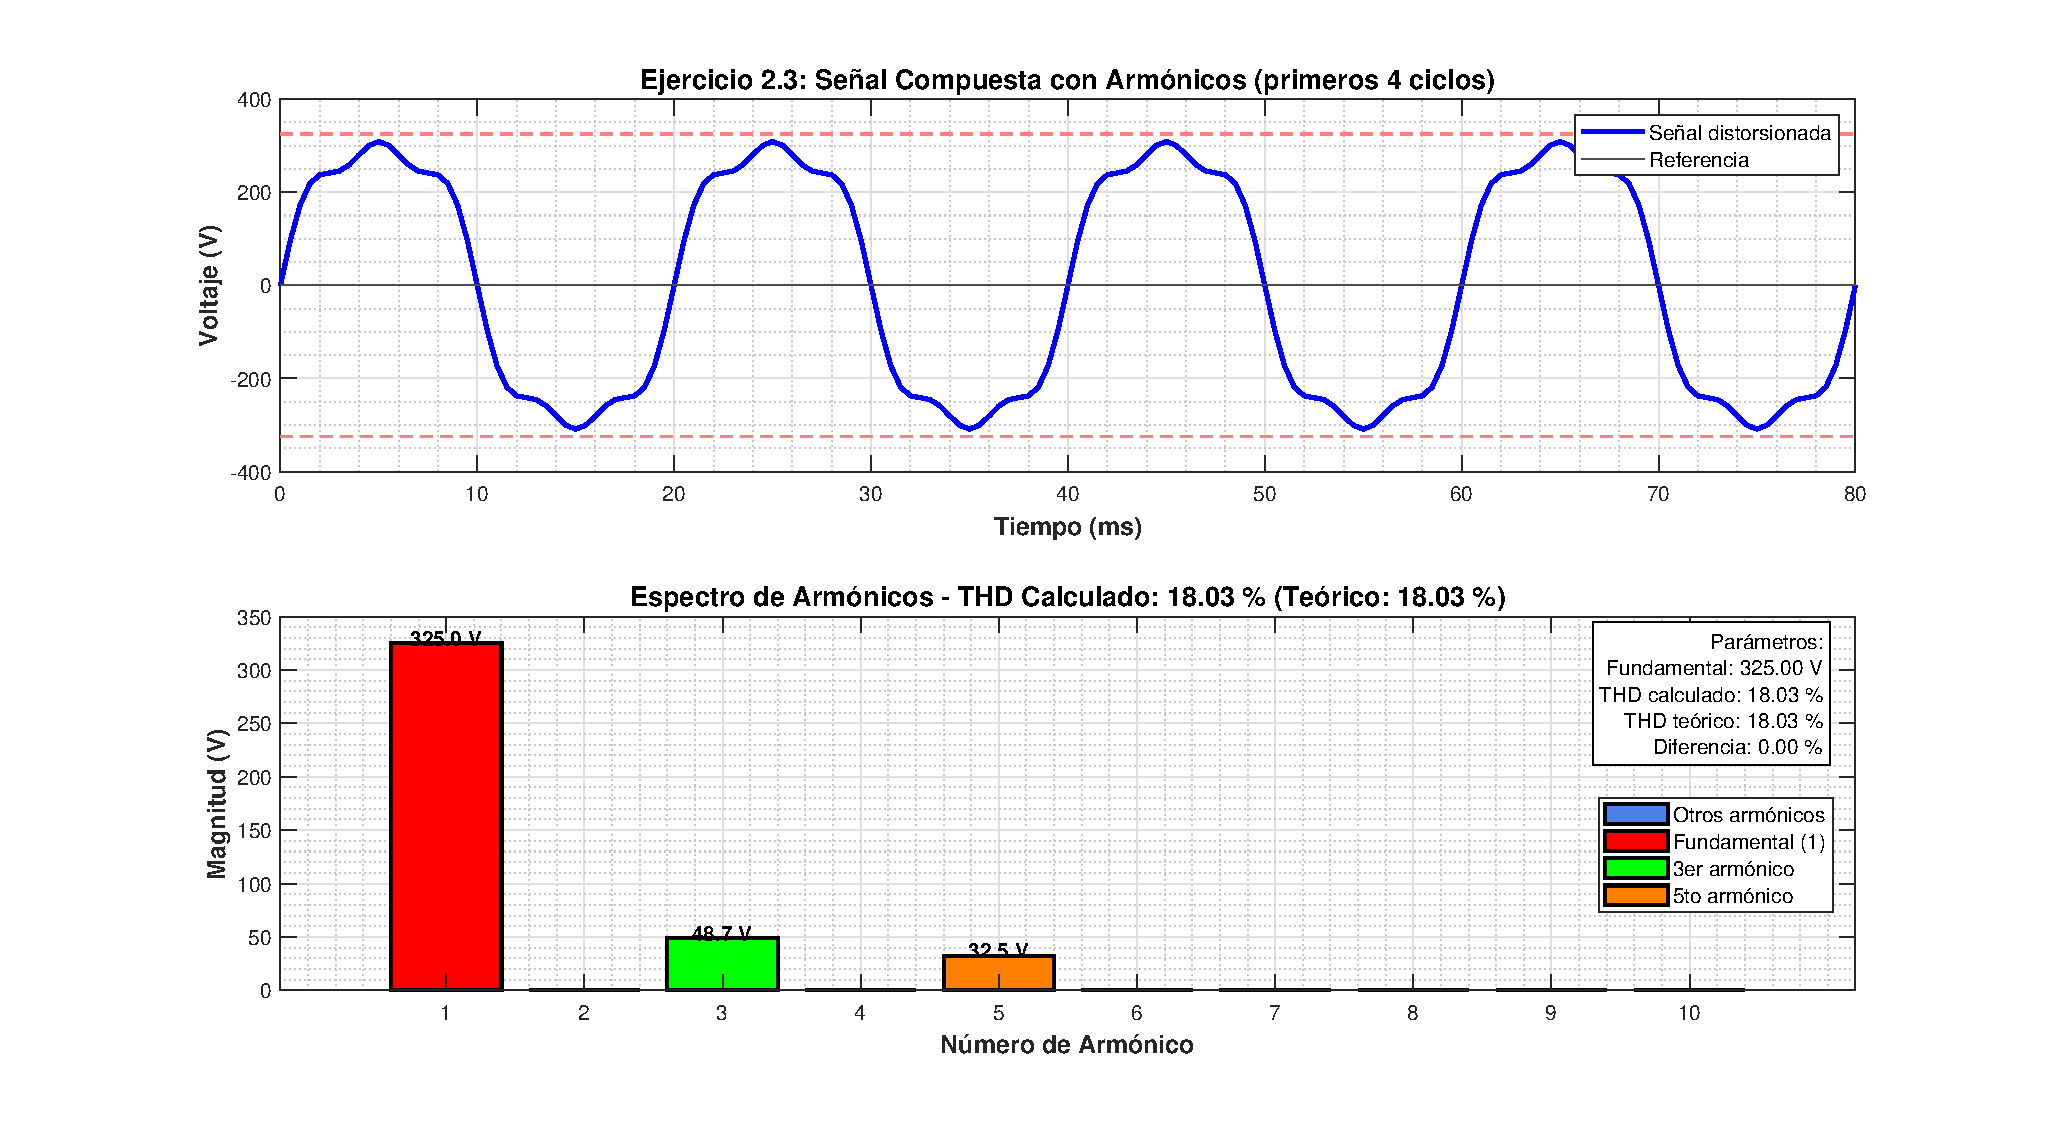
\includegraphics[width=0.99\textwidth]{grap6.eps}
  \caption{Ejercicio 2.3: Generación y análisis de señal con armónicos. La gráfica superior muestra los primeros 4 ciclos de la señal distorsionada resultante de la superposición de fundamental, 3er y 5to armónicos, observándose claramente la deformación respecto a una sinusoide pura. La gráfica inferior presenta el espectro de armónicos en barras, con colores diferenciados (rojo para fundamental, verde para 3er armónico, naranja para 5to armónico), mostrando un THD calculado de 18.03\% que supera el límite normativo del 8\%.}
  \label{fig:ejercicio2_3}
\end{figure}

\textbf{Análisis:}

El ejercicio demuestra la generación y análisis de una señal eléctrica con contenido armónico realista. La señal compuesta se obtiene mediante superposición de tres componentes sinusoidales: fundamental (50 Hz, 100\%), 3er armónico (150 Hz, 15\%) y 5to armónico (250 Hz, 10\%). Los resultados muestran una coincidencia perfecta entre el THD calculado (18.0278\%) y el teórico (18.0278\%), validando la precisión del método. La visualización temporal (primeros 4 ciclos) muestra claramente la distorsión de la forma de onda, que deja de ser sinusoidal pura. El análisis espectral revela exactamente los armónicos presentes con sus magnitudes correctas. Crítica¬mente, el THD obtenido (18.03\%) supera significativamente el límite normativo de 8\% permitido en redes de baja tensión, indicando que esta carga presenta una calidad de potencia deficiente que podría afectar negativamente a equipos sensibles conectados en la instalación.

\subsection{Actividad Guiada: Comparar Diferentes Cargas}

\begin{problembox}{Actividad Guiada - Comparación de Cargas}

\textbf{Objetivo:} Simular y comparar el contenido armónico de tres tipos de cargas.

\textbf{Cargas a simular:}

\textbf{1. Carga Lineal (ideal):}
\begin{itemize}
  \item Solo fundamental de 50 Hz
  \item Amplitud: 325 V
  \item THD esperado: $\approx 0\%$
\end{itemize}

\textbf{2. Carga con Distorsión Moderada:}
\begin{itemize}
  \item Fundamental: 325 V
  \item 3er armónico: 10\% (32.5 V)
  \item 5to armónico: 5\% (16.25 V)
  \item THD esperado: $\approx 11.2\%$
\end{itemize}

\textbf{3. Carga Altamente Distorsionada:}
\begin{itemize}
  \item Fundamental: 325 V
  \item 3er armónico: 25\% (81.25 V)
  \item 5to armónico: 15\% (48.75 V)
  \item 7mo armónico: 10\% (32.5 V)
  \item THD esperado: $\approx 30.4\%$
\end{itemize}

\textbf{Tareas:}
\begin{enumerate}
  \item Generar las tres señales con los parámetros indicados
  \item Aplicar tu función de análisis de armónicos a cada una
  \item Crear una tabla comparativa con los resultados
  \item Visualizar los espectros de las tres señales en subplots
  \item Analizar: ¿Cuál carga superaría el límite normativo del 8\%?
\end{enumerate}

\end{problembox}

\subsubsection{Solución}

\textbf{Código MATLAB:}

\begin{lstlisting}
%% ========== ACTIVIDAD GUIADA 3.4: COMPARAR DIFERENTES CARGAS ==========
clear; close all; clc;
fprintf('\n========== ACTIVIDAD GUIADA 3.4: COMPARAR DIFERENTES CARGAS ==========\n');

% Parámetros generales
fs = 2000;             % Frecuencia de muestreo (Hz)
f0 = 50;               % Frecuencia fundamental (Hz)
duracion = 1;          % Duración total (s)
t = 0:1/fs:duracion-1/fs;
Vpico = 325;           % Amplitud pico (V)

% ==========================================================
% 1. Generación de señales para tres tipos de carga
% ==========================================================

% Carga 1: Lineal (solo fundamental)
v1 = Vpico * sin(2*pi*f0*t);

% Carga 2: Distorsión moderada (3er y 5to armónico)
v2 = Vpico*sin(2*pi*f0*t) + ...
     0.10*Vpico*sin(2*pi*3*f0*t) + ...
     0.05*Vpico*sin(2*pi*5*f0*t);

% Carga 3: Altamente distorsionada (3er, 5to y 7mo)
v3 = Vpico*sin(2*pi*f0*t) + ...
     0.25*Vpico*sin(2*pi*3*f0*t) + ...
     0.15*Vpico*sin(2*pi*5*f0*t) + ...
     0.10*Vpico*sin(2*pi*7*f0*t);

% ==========================================================
% 2. Cálculo del espectro y THD
% ==========================================================

N = length(t);
f = (0:N/2-1)*(fs/N);  % Vector de frecuencias (positivas)

% Función anónima para obtener magnitud espectral
calcMag = @(v) abs(fft(v)/N)*2;

% Magnitudes
V1 = calcMag(v1);
V2 = calcMag(v2);
V3 = calcMag(v3);

% Armónicos (fundamental hasta 10º)
harmonics = 1:10;
freq_h = harmonics * f0;

% Función para extraer magnitudes de armónicos
getHarmonics = @(V) arrayfun(@(fh) ...
    V(find(abs(f - fh) == min(abs(f - fh)), 1)), freq_h);

mag1 = getHarmonics(V1);
mag2 = getHarmonics(V2);
mag3 = getHarmonics(V3);

% Cálculo del THD
THD = @(mags) 100*sqrt(sum(mags(2:end).^2))/mags(1);

THD1 = THD(mag1);
THD2 = THD(mag2);
THD3 = THD(mag3);

% ==========================================================
% 3. Resultados y tabla comparativa
% ==========================================================

fprintf('Carga Lineal (solo fundamental): THD = %.2f %%\n', THD1);
fprintf('Carga Moderadamente Distorsionada: THD = %.2f %%\n', THD2);
fprintf('Carga Altamente Distorsionada: THD = %.2f %%\n', THD3);

T = table(["Lineal"; "Moderada"; "Alta"], [THD1; THD2; THD3], ...
    'VariableNames', {'Tipo_Carga', 'THD_porcentaje'});

disp(' ');
disp('Tabla comparativa de THD:');
disp(T);

% ==========================================================
% 4. Visualización de los espectros
% ==========================================================

figure('Position', [100 100 1000 700]);

subplot(3,1,1);
stem(freq_h, mag1(1:10), 'b', 'LineWidth', 1.5);
title(sprintf('Carga Lineal - THD = %.2f %%', THD1), 'FontWeight','bold');
xlabel('Frecuencia (Hz)');
ylabel('Magnitud (V)');
grid on; xlim([0 600]);

subplot(3,1,2);
stem(freq_h, mag2(1:10), 'm', 'LineWidth', 1.5);
title(sprintf('Carga Moderada - THD = %.2f %%', THD2), 'FontWeight','bold');
xlabel('Frecuencia (Hz)');
ylabel('Magnitud (V)');
grid on; xlim([0 600]);

subplot(3,1,3);
stem(freq_h, mag3(1:10), 'r', 'LineWidth', 1.5);
title(sprintf('Carga Alta - THD = %.2f %%', THD3), 'FontWeight','bold');
xlabel('Frecuencia (Hz)');
ylabel('Magnitud (V)');
grid on; xlim([0 600]);

sgtitle('Actividad Guiada 3.4: Comparación de Espectros Armónicos', ...
    'FontWeight','bold');

% ==========================================================
% 5. Análisis final
% ==========================================================
fprintf('\nAnálisis:\n');
fprintf(['• La carga lineal tiene una señal puramente sinusoidal ' ...
    '(THD ≈ 0%%).\n']);
fprintf(['• La carga moderadamente distorsionada tiene THD ≈ %.1f%% ' ...
    '(NO CUMPLE el 8%% normativo).\n'], THD2);
fprintf(['• La carga altamente distorsionada tiene THD ≈ %.1f%% ' ...
    '(NO CUMPLE el 8%% normativo).\n\n'], THD3);

function out = ternary(cond, valTrue, valFalse)
    if cond
        out = valTrue;
    else
        out = valFalse;
    end
end
\end{lstlisting}

\textbf{Resultados:}

\begin{successbox}
\begin{itemize}
  \item \textbf{Carga Lineal:} THD = 0.00\% (Cumple normativa)
  \item \textbf{Carga Moderadamente Distorsionada:} THD = 11.18\% (NO CUMPLE)
  \item \textbf{Carga Altamente Distorsionada:} THD = 30.82\% (NO CUMPLE)
  \item \textbf{Límite normativo de referencia:} 8\% (IEC 61000-2-2)
\end{itemize}
\end{successbox}

\textbf{Tabla Comparativa:}

\begin{table}[H]
  \centering
  \begin{tabular}{|l|c|c|}
    \hline
    \textbf{Tipo de Carga} & \textbf{THD (\%)} & \textbf{Cumplimiento} \\
    \hline
    Lineal & 0.00 & ✓ CUMPLE \\
    \hline
    Moderadamente Distorsionada & 11.18 & ✗ NO CUMPLE \\
    \hline
    Altamente Distorsionada & 30.82 & ✗ NO CUMPLE \\
    \hline
  \end{tabular}
  \caption{Comparativa de THD para diferentes tipos de cargas.}
  \label{tab:comparativa_cargas}
\end{table}

\textbf{Gráfica de resultados:}

\begin{figure}[H]
  \centering
  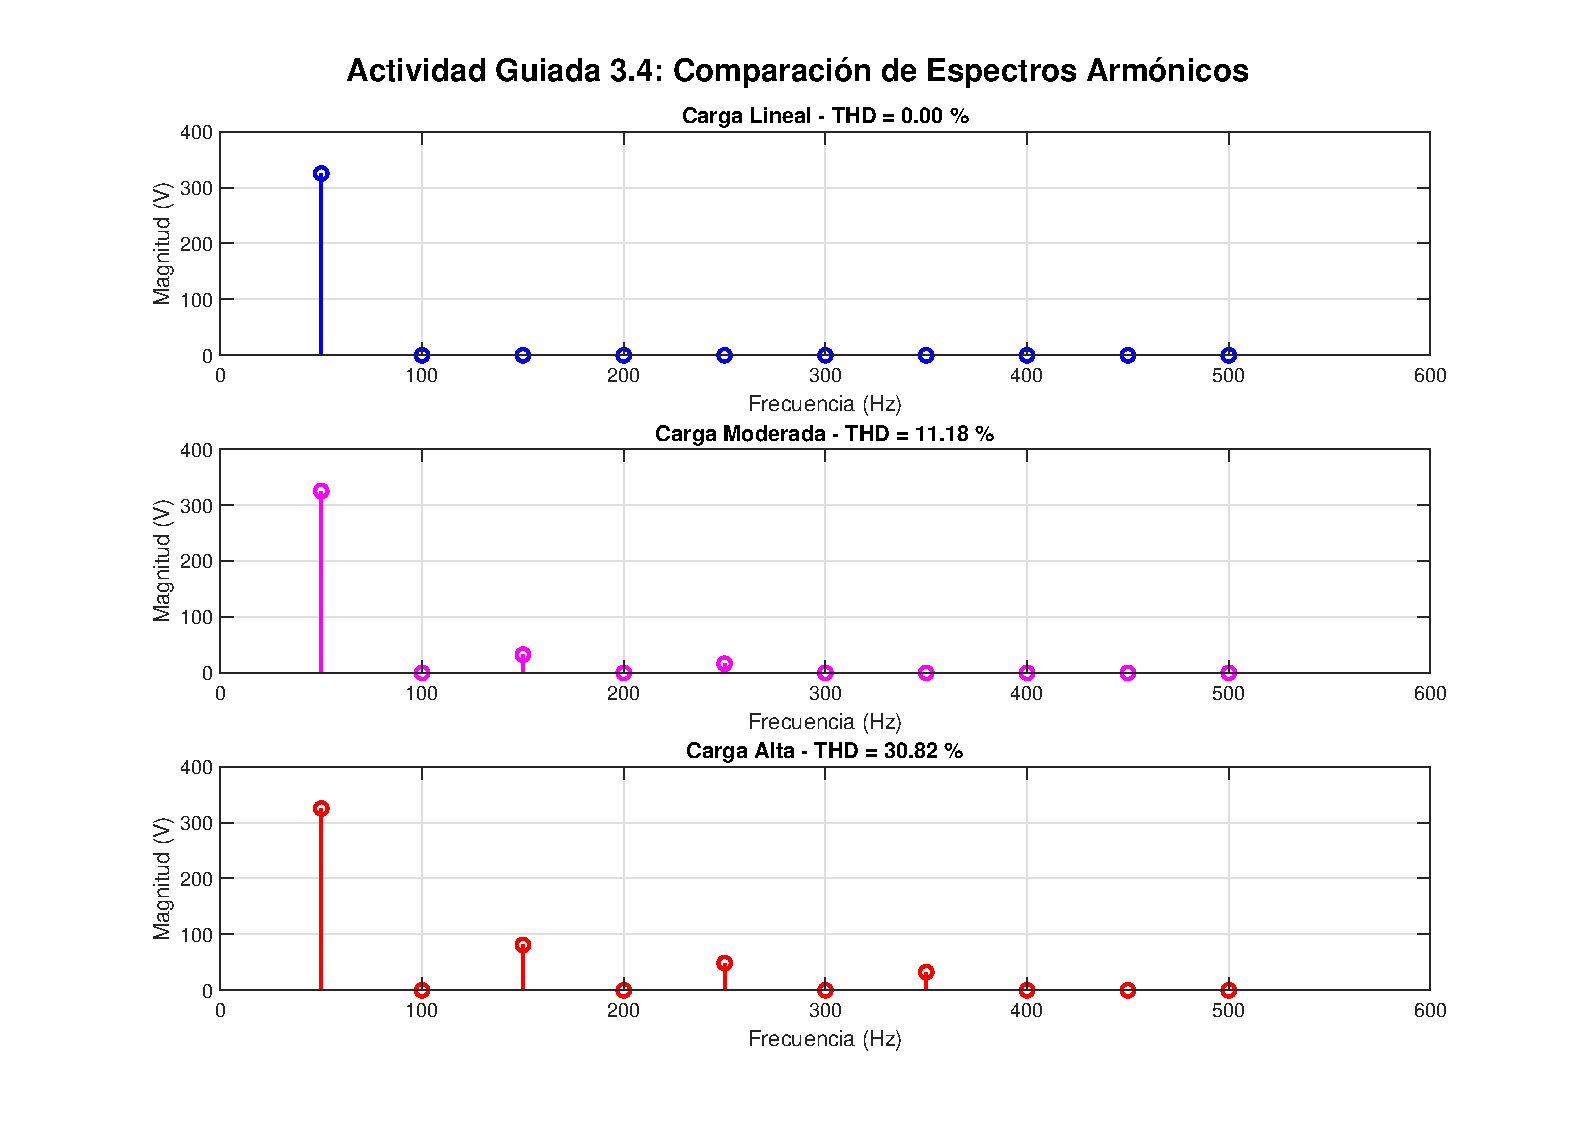
\includegraphics[width=0.99\textwidth]{grap8.eps}
  \caption{Actividad Guiada 3.4: Comparación de espectros armónicos para tres tipos de cargas. Primera fila: Carga lineal (THD = 0.00\%), mostrando únicamente el fundamental en 50 Hz. Segunda fila: Carga moderadamente distorsionada (THD = 11.18\%), con presencia de 3er y 5to armónicos. Tercera fila: Carga altamente distorsionada (THD = 30.82\%), con múltiples armónicos significativos (3er, 5to y 7mo).}
  \label{fig:actividad_comparativa_cargas}
\end{figure}

\textbf{Análisis e Interpretación:}

Este ejercicio comparativo demuestra el impacto de diferentes tipos de cargas en la calidad de la potencia eléctrica. Los resultados revelan:

\begin{infobox}
\begin{itemize}
  \item \textbf{Carga Lineal:} Proporciona una señal prácticamente perfecta (THD $\approx 0\%$), con contenido armónico negligible. Solo el fundamental en 50 Hz es significativo.
  
  \item \textbf{Carga Moderadamente Distorsionada:} Con THD del 11.18\%, esta carga ya supera el límite normativo del 8\%. Los armónicos 3º y 5º son claramente visibles en el espectro. Aunque no es la peor situación, podría causar problemas a equipos sensibles.
  
  \item \textbf{Carga Altamente Distorsionada:} Con THD del 30.82\%, esta carga presenta una contaminación armónica severa, incluyendo 3º, 5º y 7º armónicos. Constituye un riesgo significativo para la instalación eléctrica.
\end{itemize}
\end{infobox}

\textbf{Conclusión:} Las cargas \textbf{moderada} y \textbf{alta} superan el límite normativo del 8\%, siendo la carga \textbf{altamente distorsionada} la que requeriría medidas correctivas inmediatas, como la instalación de filtros pasivos o activos para reducir los armónicos a niveles aceptables. Ejemplos reales de estas cargas son convertidores electrónicos de potencia, rectificadores, variadores de velocidad y sistemas de iluminación LED de baja calidad.

\newpage

\section{Actividad Grupal: Microcortes en Data Center}

\subsection{Enunciado General}

\begin{problembox}{Grupo 5: Microcortes en Data Center}

\textbf{Escenario:} Un centro de datos experimenta microcortes que afectan a equipos críticos.

\textbf{Especificaciones de la señal:}
\begin{itemize}
  \item Duración total: 300 ms
  \item Tensión nominal: 325 V pico
  \item Eventos:
  \begin{itemize}
    \item Microcorte 1: Hueco del 80\% durante 15 ms (inicio: 50 ms)
    \item Microcorte 2: Hueco del 70\% durante 20 ms (inicio: 150 ms)
  \end{itemize}
\end{itemize}

\end{problembox}

\subsection{Tareas Específicas}

\begin{problembox}{Tareas del Grupo 5}

Las tareas a realizar son las siguientes:

\begin{enumerate}
  \item Generar la señal con ambos microcortes
  \item Calcular RMS deslizante (ventana: 10 ms)
  \item Identificar y caracterizar ambos eventos
  \item Clasificar los huecos según la norma IEC 61000-4-11
  \item Determinar si un UPS con tiempo de conmutación de 4 ms protegería adecuadamente
  \item Justificar la respuesta con datos del análisis
\end{enumerate}

\end{problembox}



El escenario propuesto corresponde a un centro de datos que experimenta microcortes que afectan a equipos críticos de procesamiento y almacenamiento de información. Este tipo de instalaciones son especialmente sensibles a las perturbaciones en el suministro eléctrico debido a la naturaleza crítica de sus operaciones y a los estrictos requisitos de disponibilidad que deben cumplir. Los microcortes, aunque breves en duración, pueden causar reinicios de servidores, pérdida de datos en memoria y desconexiones de equipos de red, comprometiendo la continuidad del servicio.

Para el análisis se ha generado una señal eléctrica sintética que reproduce las condiciones reales del escenario descrito. La señal simulada tiene una duración total de 300 milisegundos con una tensión nominal de 325 V de amplitud pico, correspondiente a una red monofásica estándar europea de 230 V eficaces y 50 Hz de frecuencia. Sobre esta señal base se han superpuesto dos eventos de microcorte con características específicas. El primer microcorte se produce a los 50 milisegundos del inicio de la medición, presenta una profundidad del 80\%, es decir, la tensión se reduce hasta el 20\% de su valor nominal, y tiene una duración de 15 milisegundos. El segundo microcorte ocurre a los 150 milisegundos, alcanza una profundidad del 70\%, reduciendo la tensión al 30\% del valor nominal, y se extiende durante 20 milisegundos.

\begin{figure}[htbp]
\centering
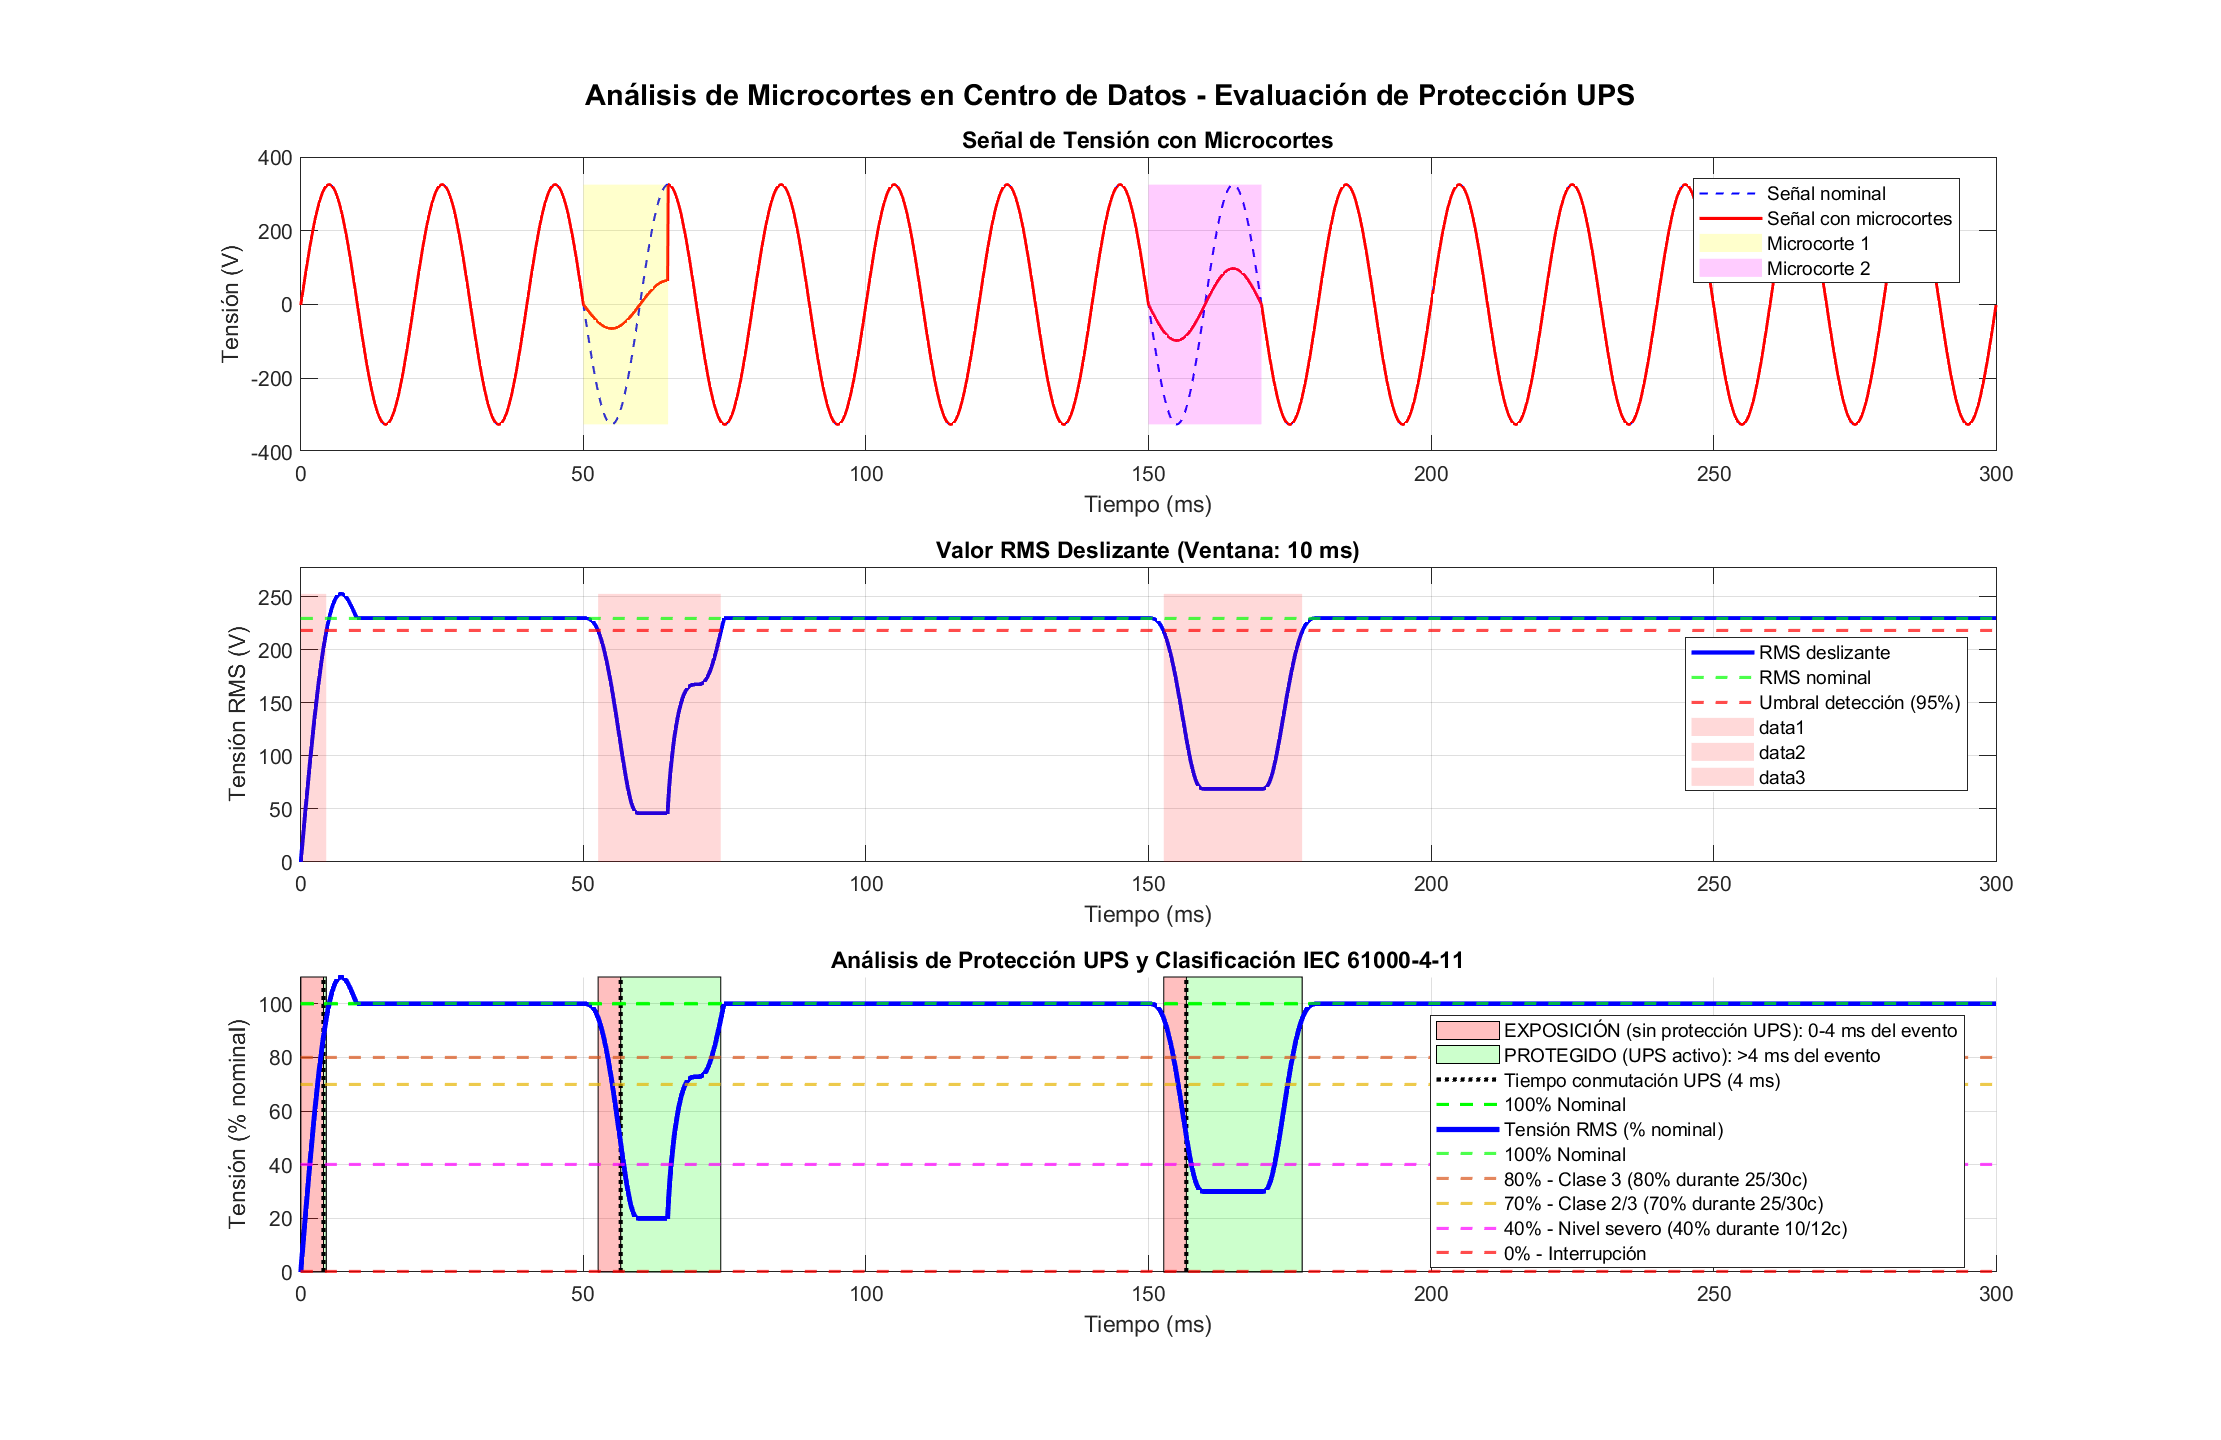
\includegraphics[width=1\textwidth]{figures/microcortes_datacenter.eps}
\caption{Análisis completo de microcortes en centro de datos. Superior: señal de tensión con eventos marcados. Centro: valor RMS deslizante con ventana de 10 milisegundos. Inferior: análisis de protección UPS y clasificación según IEC 61000-4-11.}
\label{fig:microcortes}
\end{figure}


El análisis de la señal generada se ha realizado mediante el cálculo del valor eficaz o RMS en ventanas deslizantes de diez milisegundos. Esta longitud de ventana ha sido seleccionada específicamente conforme a la norma IEC 61000-4-30 (Clase A), que especifica una resolución temporal de 10 ms para la medición de parámetros de calidad de energía. Esta resolución permite capturar adecuadamente la dinámica de eventos de corta duración como los microcortes, que típicamente duran entre unos pocos milisegundos y varias decenas de milisegundos. Una ventana más amplia, como los veinte milisegundos correspondientes a un ciclo completo de la red, proporcionaría una respuesta más suavizada pero con menor capacidad de detección precisa del inicio y fin de los eventos. Por el contrario, una ventana excesivamente pequeña introduciría fluctuaciones espurias debido al contenido fundamental de la señal sinusoidal.

Los resultados del análisis RMS deslizante muestran claramente la detección de ambos microcortes. El primer evento reduce el valor eficaz desde el valor nominal de 229.81 V hasta aproximadamente 46 V, lo que representa una tensión residual del 20\%. Esta reducción tan severa se mantiene durante toda la duración del microcorte y el sistema de análisis captura tanto el flanco de bajada inicial como la recuperación posterior. Por su parte, el segundo evento presenta una reducción hasta aproximadamente 69 V, correspondiente a una tensión residual del 30\%. La duración ligeramente superior de este segundo evento (20 ms frente a 15 ms) también queda reflejada en el análisis temporal del valor RMS. El tiempo de recuperación, medido desde el final del hueco hasta que el valor RMS vuelve a estar dentro del 10\% del valor nominal, es de aproximadamente un ciclo completo de la red (20 ms adicionales). Esta característica de recuperación gradual es inherente al método de cálculo del RMS deslizante con ventana finita.

Para contextualizar la gravedad de estos eventos se ha realizado la clasificación según la norma IEC 61000-4-11, que establece los métodos de prueba y niveles de inmunidad que deben tener los equipos eléctricos y electrónicos conectados a redes de baja tensión frente a huecos de tensión, interrupciones breves y variaciones de tensión. La norma IEC 61000-4-11 define diferentes clases de equipos que deben superar niveles de prueba específicos. La Clase 1 se define caso por caso según los requisitos específicos de cada equipo particular. La Clase 2 es aplicable a equipos conectados a redes públicas y entornos comerciales, incluyendo niveles de prueba como 0\% durante medio periodo (10 ms a 50 Hz), 0\% durante un periodo completo (20 ms a 50 Hz), y 70\% de tensión residual durante 25 a 30 periodos (500 ms a 50 Hz). La Clase 3 se aplica a entornos industriales con requisitos más exigentes, contemplando 0\% durante medio periodo (10 ms), 0\% durante un periodo (20 ms), 40\% de tensión residual durante 10 a 12 periodos (200 ms a 50 Hz), 70\% durante 25 a 30 periodos (500 ms), y 80\% durante 250 a 300 periodos (5 segundos a 50 Hz). Finalmente, la Clase X queda especificada por el fabricante o usuario para aplicaciones especiales que no se ajustan a las clases estándar. Es importante señalar que el término ``0\% durante'' en las tablas de la norma significa que al inicio del hueco la tensión cae instantáneamente, no que permanece a 0\% durante todo el evento. El porcentaje especificado (40\%, 70\%, 80\%) indica la tensión residual que permanece durante el hueco.

El primer evento analizado presenta una duración de 15 milisegundos, equivalente a 0.75 periodos a 50 Hz, con una tensión residual del 20\% (46 V RMS), lo que implica una reducción del 80\%. Este evento se clasifica como hueco de tensión según la Tabla 1 de IEC 61000-4-11. Al comparar este evento con los niveles de prueba normalizados, se observa que la duración se sitúa entre las pruebas de medio periodo (10 ms) y un periodo completo (20 ms) contempladas en las Clases 2 y 3. Sin embargo, la profundidad del hueco es significativamente mayor que cualquier nivel estándar. La Clase 2 requiere una tensión residual de al menos 70\%, requisito que no se cumple ya que 20\% es muy inferior a 70\%. Asimismo, la Clase 3 requiere una tensión residual de al menos 40\% para huecos cortos, y nuevamente el evento no cumple este requisito al presentar solo un 20\% de tensión residual. Por tanto, este evento supera en severidad todos los niveles de prueba estándar de las Clases 2 y 3, clasificándose como Clase X (especial), lo que requiere análisis y especificaciones particulares. La severidad del evento se considera muy alta, dado que un equipo certificado Clase 2 o Clase 3 no está garantizado para operar correctamente ante este evento, ya que la profundidad del hueco excede los niveles de prueba normalizados.

El segundo evento presenta una duración de 20 milisegundos, equivalente a un periodo completo a 50 Hz, con una tensión residual del 30\% (69 V RMS), lo que representa una reducción del 70\%. Este evento también se clasifica como hueco de tensión según la Tabla 1 de IEC 61000-4-11. La duración de este evento coincide exactamente con una de las pruebas estándar (un periodo completo), sin embargo, la profundidad del hueco sigue siendo superior a los niveles normalizados. La Clase 2 requiere una tensión residual de al menos 70\% para eventos de un periodo, y este evento con 30\% no cumple este requisito. De igual manera, la Clase 3 requiere una tensión residual de al menos 40\% para huecos cortos, y el evento tampoco cumple al presentar solo un 30\%. Aunque la duración coincide con los niveles de prueba estándar, la profundidad del hueco (30\% residual) es más severa que los requisitos de Clase 2 (70\%) y Clase 3 (40\%), por lo que debe clasificarse igualmente como Clase X (especial). La severidad se considera alta, dado que un equipo certificado para soportar huecos de un periodo según Clase 2 o 3 podría fallar porque el hueco es más profundo que los niveles especificados en las pruebas de certificación.

El análisis detallado de ambos microcortes detectados revela que superan los niveles de prueba establecidos en las Clases 2 y 3 de la norma IEC 61000-4-11, por lo que requieren equipos con especificaciones Clase X (especiales). Esta clasificación implica que los equipos estándar certificados conforme a las clases regulares no están garantizados para operar correctamente durante estos eventos, demandando por tanto sistemas de protección adicionales, como los UPS, debido a su severidad. Estos eventos están dentro del rango de perturbaciones esperables según la norma EN 50160, que establece una frecuencia típica de 5 a 50 eventos anuales para huecos con profundidades superiores al 60\%. La norma establece que los equipos conectados a redes públicas deben ser capaces de soportar los eventos correspondientes a sus clases de certificación, o en su defecto, contar con sistemas de protección apropiados como los UPS. En este caso particular, dado que los eventos superan las clases estándar y se clasifican como Clase X, la protección mediante UPS no es opcional sino obligatoria para garantizar la continuidad operativa del centro de datos.

Un aspecto fundamental del análisis es la evaluación de la efectividad de un sistema de alimentación ininterrumpida (UPS) como medida de protección. El sistema analizado corresponde a un UPS de tipo Off-line (VFD - Voltage and Frequency Dependent según IEC 62040-3) con un tiempo de conmutación de 4 milisegundos, operando normalmente en modo bypass y conmutando a baterías cuando se detecta un fallo en el suministro eléctrico.

\begin{table}[h]
\centering
\begin{tabular}{|l|c|c|}
\hline
\textbf{Parámetro} & \textbf{Valor} & \textbf{Evaluación} \\
\hline
Duración del evento & 15 ms & Mayor que t$_{\text{conm}}$ \\
Tiempo de conmutación UPS & 4 ms & - \\
Tiempo de exposición & 4 ms & 27\% del evento \\
Tiempo protegido & 11 ms & 73\% del evento \\
Profundidad del hueco & 80\% & Crítica \\
\hline
\end{tabular}
\caption{Análisis de protección UPS para el Evento 1}
\end{table}

Durante los primeros 4 milisegundos, el equipo queda expuesto directamente al hueco del 80\% (tensión del 20\%). Aunque muchas fuentes de alimentación modernas tienen capacidad de hold-up (condensadores internos) de 10-20 ms, un hueco tan profundo puede comprometer esta capacidad. Después de 4 ms, el UPS conmuta y proporciona alimentación estable desde baterías durante los 11 ms restantes, configurando una protección parcial con riesgo medio-alto.

\begin{table}[h]
\centering
\begin{tabular}{|l|c|c|}
\hline
\textbf{Parámetro} & \textbf{Valor} & \textbf{Evaluación} \\
\hline
Duración del evento & 20 ms & Mayor que t$_{\text{conm}}$ \\
Tiempo de conmutación UPS & 4 ms & - \\
Tiempo de exposición & 4 ms & 20\% del evento \\
Tiempo protegido & 16 ms & 80\% del evento \\
Profundidad del hueco & 70\% & Alta \\
\hline
\end{tabular}
\caption{Análisis de protección UPS para el Evento 2}
\end{table}

El equipo está expuesto durante los primeros 4 milisegundos al hueco del 70\% (tensión del 30\%). Aunque menos severo que el primer evento, sigue siendo una perturbación significativa. Después de la conmutación, el UPS proporciona protección durante los 16 ms restantes (80\% del evento), resultando en una protección parcial con riesgo medio.

En la gráfica inferior de la Figura \ref{fig:microcortes} se han representado mediante código de colores las zonas de protección del UPS. Las zonas rojas corresponden a los periodos de exposición sin protección (primeros 4 ms de cada evento), durante los cuales el equipo recibe directamente la tensión degradada de la red. Las zonas verdes representan los periodos con protección UPS activa (después de 4 ms del inicio de cada evento), cuando el equipo recibe alimentación estable desde las baterías del UPS. Las líneas verticales punteadas marcan el instante preciso de conmutación del UPS, que ocurre 4 milisegundos después del inicio de cada evento detectado.

Es importante considerar varios factores que afectan la efectividad real de la protección. En primer lugar, los servidores y sistemas de almacenamiento modernos cuentan con fuentes de alimentación switching equipadas con condensadores internos que pueden mantener la alimentación durante un periodo típico de 10 a 20 milisegundos, conocido como hold-up time. Sin embargo, un hueco del 80\% puede reducir significativamente esta capacidad de sostén de energía. Por otra parte, el tiempo de conmutación nominal de 4 milisegundos puede verse afectado por factores externos como la temperatura ambiente, el envejecimiento de los componentes electrónicos y el nivel de carga conectada al UPS, pudiendo incrementarse en condiciones adversas. Adicionalmente, la efectividad de la protección depende críticamente de que el UPS se encuentre operativo, correctamente mantenido y con su batería suficientemente cargada. Si el UPS presenta algún fallo o las baterías están degradadas, la protección no será efectiva. Finalmente, deben considerarse los efectos acumulativos de múltiples eventos en corto tiempo, ya que los condensadores de las fuentes de alimentación pueden no recuperarse completamente entre eventos sucesivos, aumentando el riesgo de fallo.

El UPS con tiempo de conmutación de 4 milisegundos proporciona protección parcial pero no adecuada para un centro de datos crítico. Esta conclusión se fundamenta en varios aspectos críticos. En primer lugar, los equipos quedan expuestos durante 4 milisegundos, lo que representa un 27\% de la duración total del primer evento y un 20\% del segundo evento, enfrentándose a huecos muy severos de 70 a 80\% de profundidad. En segundo lugar, ambos eventos superan los niveles de prueba establecidos en las Clases 2 y 3 de la norma IEC 61000-4-11, clasificándose como eventos Clase X (especiales), lo que indica una severidad extrema que excede las condiciones normalizadas. Durante el tiempo de exposición pueden ocurrir diversos tipos de fallos en los equipos críticos, incluyendo reinicios inesperados de servidores, pérdida de datos almacenados en memoria volátil, desconexiones de equipos de red activos, y corrupción de operaciones de escritura en disco que estén en curso durante el evento. Finalmente, la criticidad inherente al entorno de un centro de datos, que requiere niveles de disponibilidad del 99.99\% o superiores, hace que cualquier interrupción, por breve que sea, tenga consecuencias económicas y reputacionales significativas para la organización.

Desde el punto de vista del análisis temporal, el primer evento tiene una duración total de 15 milisegundos, de los cuales el equipo está expuesto durante 4 ms (27\% del tiempo total) y protegido durante 11 ms (73\% restante). El segundo evento dura 20 milisegundos en total, con 4 ms de exposición (20\%) y 16 ms de protección (80\%). Aunque el porcentaje de tiempo protegido es elevado, el periodo de exposición inicial es suficientemente largo como para comprometer la operación de equipos sensibles. Desde la perspectiva normativa, ambos eventos han sido clasificados como Clase X al estar fuera de los estándares regulares. Las profundidades de 70\% y 80\% de reducción superan ampliamente los niveles establecidos para Clase 2 (70\% de tensión residual) y Clase 3 (40\% de tensión residual). Esta clasificación implica que los equipos certificados según las clases estándar no garantizan una operación correcta durante estos eventos, requiriendo medidas de protección adicionales específicamente diseñadas para estas condiciones severas. El análisis de riesgo revela que, según la norma EN 50160, la frecuencia esperada de eventos con profundidades superiores al 60\% se sitúa entre 5 y 50 eventos por año. Cada evento individual tiene un impacto medio-alto con pérdida potencial del servicio. El riesgo acumulado se considera alto, dado que la ocurrencia de múltiples eventos a lo largo del año puede causar fallos repetidos y degradación progresiva de los sistemas, afectando significativamente la disponibilidad global del centro de datos.

Para garantizar la protección adecuada de los equipos críticos del centro de datos, se propone como solución óptima la implementación de un UPS Online de doble conversión. Este sistema, clasificado como topología VFI (Voltage and Frequency Independent según IEC 62040-3), presenta un tiempo de transferencia de 0 milisegundos al no requerir conmutación, ya que realiza conversión continua de AC a DC y nuevamente a AC. Esta configuración proporciona protección del 100\% contra ambos eventos detectados, ofreciendo además ventajas adicionales como filtrado completo de perturbaciones eléctricas, regulación perfecta de tensión y frecuencia, y ausencia de tiempo muerto durante transiciones. Esta solución es específicamente recomendada para datacenters críticos debido a su elevada fiabilidad y protección total.

El análisis realizado demuestra que los microcortes detectados en el centro de datos, aunque breves (15-20 ms), son lo suficientemente severos (70-80\% de reducción) como para superar los niveles de prueba estándar de la norma IEC 61000-4-11 y clasificarse como eventos Clase X (especiales). Un UPS con tiempo de conmutación de 4 ms proporciona protección parcial pero insuficiente para un entorno crítico, dejando los equipos expuestos durante periodos significativos (4 ms = 20-27\% de la duración total de cada evento). Para garantizar la continuidad operativa del centro de datos, se requiere implementar un \textbf{UPS Online (doble conversión)} con tiempo de transferencia de 0 ms, que proporcione protección total contra estos eventos. La inversión en protección adecuada es crítica para evitar pérdida de datos, tiempo de inactividad costoso, daños en equipos y pérdida de reputación del servicio.




\subsection{Formato de Entrega}

\begin{infobox}

El trabajo debe incluir:

\begin{enumerate}
  \item \textbf{Código MATLAB:}
  \begin{itemize}
    \item Funciones implementadas (correctamente comentadas)
    \item Script principal de análisis
    \item Código para generación de gráficas
  \end{itemize}
  
  \item \textbf{Informe Técnico (máximo 10 páginas):}
  \begin{itemize}
    \item Introducción al problema específico
    \item Metodología de análisis empleada
    \item Resultados con gráficas claras y bien etiquetadas
    \item Análisis e interpretación de resultados
    \item Conclusiones y recomendaciones técnicas
  \end{itemize}
  
  \item \textbf{Gráficas Requeridas:}
  \begin{itemize}
    \item Señal temporal completa
    \item Zoom de los eventos más relevantes
    \item RMS deslizante (si aplica)
    \item Espectro de frecuencias (si aplica)
    \item Gráfico de barras de armónicos (si aplica)
  \end{itemize}
\end{enumerate}

\end{infobox}

\newpage

\section*{Repositorio del Proyecto}
El código completo de este proyecto está disponible públicamente en el siguiente repositorio de GitHub:

\begin{center}
\url{https://github.com/pgm691/Itinerario_Electrica_Grupo5_2}
\end{center}

El repositorio contiene toda la documentación necesaria para reproducir las simulaciones y análisis presentados en este trabajo.

\end{document}